% THIS IS SIGPROC-SP.TEX - VERSION 3.1
% WORKS WITH V3.2SP OF ACM_PROC_ARTICLE-SP.CLS
% APRIL 2009
%
% It is an example file showing how to use the 'acm_proc_article-sp.cls' V3.2SP
% LaTeX2e document class file for Conference Proceedings submissions.
% ----------------------------------------------------------------------------------------------------------------
% This .tex file (and associated .cls V3.2SP) *DOES NOT* produce:
%       1) The Permission Statement
%       2) The Conference (location) Info information
%       3) The Copyright Line with ACM data
%       4) Page numbering
% ---------------------------------------------------------------------------------------------------------------
% It is an example which *does* use the .bib file (from which the .bbl file
% is produced).
% REMEMBER HOWEVER: After having produced the .bbl file,
% and prior to final submission,
% you need to 'insert'  your .bbl file into your source .tex file so as to provide
% ONE 'self-contained' source file.
%
% Questions regarding SIGS should be sent to
% Adrienne Griscti ---> griscti@acm.org
%
% Questions/suggestions regarding the guidelines, .tex and .cls files, etc. to
% Gerald Murray ---> murray@hq.acm.org
%
% For tracking purposes - this is V3.1SP - APRIL 2009

\documentclass{acm_proc_article-sp}

% allows for temporary adjustment of side margins
\usepackage{chngpage}

% just makes the table prettier (see \toprule, \bottomrule, etc. commands below)
\usepackage{booktabs}

\usepackage[utf8]{inputenc}
%\usepackage[font=small,skip=0pt]{caption}

% footnotes
\usepackage{scrextend}

% URL handling
\usepackage{url}
\urlstyle{same}

% Todos
%\usepackage[colorinlistoftodos]{todonotes}
%\newcommand{\ke}[1]{\todo[size=\small, color=orange!40]{\textbf{Kai:} #1}}
%\newcommand{\tb}[1]{\todo[size=\small, color=green!40]{\textbf{Thomas:} #1}}

%\usepackage{makeidx}  % allows for indexgeneration

%\usepackage{amsmath}
\usepackage{amsmath, amssymb}
\usepackage{mathabx}
\usepackage{caption} 
\captionsetup[table]{skip=10pt}

% monospace within text
\newcommand{\ms}[1]{%
  \texttt{#1}
}

% examples
\usepackage{fancyvrb}
\DefineVerbatimEnvironment{ex}{Verbatim}{numbers=left,numbersep=2mm,frame=single,fontsize=\scriptsize}

\usepackage{xspace}
% Einfache und doppelte Anfuehrungszeichen
\newcommand{\qs}{``} 
\newcommand{\qe}{''\xspace} 
\newcommand{\sqs}{`} 
\newcommand{\sqe}{'\xspace} 

% checkmark
\usepackage{tikz}
\def\checkmark{\tikz\fill[scale=0.4](0,.35) -- (.25,0) -- (1,.7) -- (.25,.15) -- cycle;} 

% Xs
\usepackage{pifont}

% Tabellenabstände kleiner
\setlength{\intextsep}{10pt} % Vertical space above & below [h] floats
\setlength{\textfloatsep}{10pt} % Vertical space below (above) [t] ([b]) floats
% \setlength{\abovecaptionskip}{0pt}
% \setlength{\belowcaptionskip}{0pt}

\usepackage{tabularx}
\newcommand{\hr}{\hline\noalign{\smallskip}} % für die horizontalen linien in tabellen

% Todos
\usepackage[colorinlistoftodos]{todonotes}
\newcommand{\ke}[1]{\todo[size=\small, color=orange!40]{\textbf{Kai:} #1}}
\newcommand{\tb}[1]{\todo[size=\small, color=green!40]{\textbf{Thomas:} #1}}
\newcommand{\er}[1]{\todo[size=\small, color=red!40]{\textbf{Erman:} #1}}
\newcommand{\an}[1]{\todo[size=\small, color=blue!40]{\textbf{Andy:} #1}}

\newenvironment{table-1cols}{
  \scriptsize
  \sffamily
  \vspace{0.3cm}
  \begin{tabular}{l}
  \hline
  \textbf{Requirements} \\
  \hline

}{
  \hline
  \end{tabular}
  \linebreak
}

\newenvironment{table-2cols}{
  \scriptsize
  \sffamily
  \vspace{0.3cm}
  \begin{tabular}{l|l}
  \hline
  \textbf{Requirements} & \textbf{Covering DSCLs} \\
  \hline

}{
  \hline
  \end{tabular}
  \linebreak
}

\newenvironment{complexity}{
  %\scriptsize
  %\sffamily
  %\vspace{0.3cm}
  \begin{tabular}{l|l}
  \hline
  \textbf{Complexity Class} & \textbf{Complexity} \\
  \hline

}{
  \hline
  \end{tabular}
  \linebreak
}

\newenvironment{DL}{
  %\scriptsize
  %\sffamily
  \vspace{0cm}
  \begin{tabular}{l l}

}{
  \end{tabular}
  %\linebreak
}


\newenvironment{evaluation}{
  %\scriptsize
  %\sffamily
  %\vspace{0.3cm}
  \begin{tabular}{l|c|c|c|c|c|c}
  \hline
  \textbf{Constraint Class} & \textbf{DSP} & \textbf{OWL2-DL} & \textbf{OWL2-QL} & \textbf{ReSh} & \textbf{ShEx} & \textbf{SPIN} \\
  \hline

}{
  \hline
  \end{tabular}
  \linebreak
}

\newenvironment{constraint-languages-complexity}{
  %\scriptsize
  %\sffamily
  %\vspace{0.3cm}
  \begin{tabular}{l|c|c|c|c|c|c}
  \hline
  \textbf{Complexity Class} & \textbf{DSP} & \textbf{OWL2-DL} & \textbf{OWL2-QL} & \textbf{ReSh} & \textbf{ShEx} & \textbf{SPIN} \\
  \hline

}{
  \hline
  \end{tabular}
  \linebreak
}

\newenvironment{user-fiendliness}{
  %\scriptsize
  %\sffamily
  %\vspace{0.3cm}
  \begin{tabular}{l|c|c|c|c|c}
  \hline
  \textbf{criterion} & \textbf{DSP} & \textbf{OWL2} & \textbf{ReSh} & \textbf{ShEx} & \textbf{SPIN} \\
  \hline

}{
  \hline
  \end{tabular}
  \linebreak
}

\usepackage{float}

\begin{document}

%\title{The Role of Constraint Languages and Reasoning for RDF Validation}
\title{The Role of Reasoning for RDF Validation}
% On Constraint Languages for RDF Validation with an account to Reasoning
%On Constraint Languages for RDF Validation and Reasoning
%RDF Validation - Classification of Constraints and Constraint Languages According to Reasoning, Expressivity, and Complexity
%RDF Validation: An Analysis of Constraint Languages
%Analysing Constraint Languages for RDF Validation
%Classifying Constraint Languages for RDF Validation
%RDF Validation and Reasoning.
%Classifying Constraint Languages for RDF validation Concerning Reasoning
%
% You need the command \numberofauthors to handle the 'placement
% and alignment' of the authors beneath the title.
%
% For aesthetic reasons, we recommend 'three authors at a time'
% i.e. three 'name/affiliation blocks' be placed beneath the title.
%
% NOTE: You are NOT restricted in how many 'rows' of
% "name/affiliations" may appear. We just ask that you restrict
% the number of 'columns' to three.
%
% Because of the available 'opening page real-estate'
% we ask you to refrain from putting more than six authors
% (two rows with three columns) beneath the article title.
% More than six makes the first-page appear very cluttered indeed.
%
% Use the \alignauthor commands to handle the names
% and affiliations for an 'aesthetic maximum' of six authors.
% Add names, affiliations, addresses for
% the seventh etc. author(s) as the argument for the
% \additionalauthors command.
% These 'additional authors' will be output/set for you
% without further effort on your part as the last section in
% the body of your article BEFORE References or any Appendices.

\numberofauthors{4} %  in this sample file, there are a *total*
% of EIGHT authors. SIX appear on the 'first-page' (for formatting
% reasons) and the remaining two appear in the \additionalauthors section.
%
\author{
% You can go ahead and credit any number of authors here,
% e.g. one 'row of three' or two rows (consisting of one row of three
% and a second row of one, two or three).
%
% The command \alignauthor (no curly braces needed) should
% precede each author name, affiliation/snail-mail address and
% e-mail address. Additionally, tag each line of
% affiliation/address with \affaddr, and tag the
% e-mail address with \email.
%
% 1st. author
\alignauthor
Thomas Bosch\\
       \affaddr{GESIS - Leibniz Institute for the Social Sciences, Germany}\\
       %\affaddr{1932 Wallamaloo Lane}\\
       %\affaddr{Wallamaloo, New Zealand}\\
       \email{thomas.bosch@gesis.org}
% 2nd. author
\alignauthor
Erman Acar\\
       \affaddr{University of Mannheim, Germany}\\
       %\affaddr{P.O. Box 1212}\\
       %\affaddr{Dublin, Ohio 43017-6221}\\
       \email{erman@informatik.uni-mannheim.de}
% 3rd. author
\alignauthor Andreas Nolle\\
       \affaddr{Albstadt-Sigmaringen University, Germany}\\
       %\affaddr{1 Th{\o}rv{\"a}ld Circle}\\
       %\affaddr{Hekla, Iceland}\\
       \email{nolle@hs-albsig.de}
\and  % use '\and' if you need 'another row' of author names
% 4th. author
\alignauthor Kai Eckert\\
       \affaddr{Stuttgart Media University, Germany}\\
       %\affaddr{Brookhaven National Lab}\\
       %\affaddr{P.O. Box 5000}\\
       \email{eckert@hdm-stuttgart.de}
}
% There's nothing stopping you putting the seventh, eighth, etc.
% author on the opening page (as the 'third row') but we ask,
% for aesthetic reasons that you place these 'additional authors'
% in the \additional authors block, viz.
%\additionalauthors{Additional authors: John Smith (The Th{\o}rv{\"a}ld Group,
%email: {\texttt{jsmith@affiliation.org}}) and Julius P.~Kumquat
%(The Kumquat Consortium, email: {\texttt{jpkumquat@consortium.net}}).}
%\date{30 July 1999}
% Just remember to make sure that the TOTAL number of authors
% is the number that will appear on the first page PLUS the
% number that will appear in the \additionalauthors section.

\maketitle
\begin{abstract}
For data practitioners embracing the world of RDF and Linked Data, the openness and flexibility is a mixed blessing. 
For them, data validation according to predefined constraints is a much sought-after feature, particularly as this is taken for granted in the XML world.

We investigate the role that reasoning plays in practical data validation and 
how to overcome the major shortcomings when validating RDF data by performing reasoning prior to validation.
Based on our work in the DCMI RDF Application Profiles Task Group and in cooperation with the W3C Data Shapes Working Group, 
we identified and published by today 81 types of constraints that are required by various stakeholders for data applications. 
For each constraint type we examine
(1) if validation results depend on different underlying semantics,
(2) if reasoning may improve data quality, and 
(3) how efficient in terms of runtime validation is performed with and without reasoning.
Using these findings, we determine for the most common constraint languages which constraint types they are able to express.
We argue that so far no single best solution exists and give directions for the further development of constraint languages.
%\begin{abstract}
%For data practitioners embracing the world of RDF and Linked Data, the openness and flexibility is a mixed blessing. For them, data validation according to predefined constraints is a  much sought-after feature, particularly as this is taken for granted in the XML world. 
%Several languages exist to meet this requirement, ranging from using \emph{OWL} as a constraint language to \emph{SPIN}, a SPARQL-based way to formulate and check constraints. 
%In this paper, we investigate the relationship of validation and reasoning and the role that reasoning plays in practical data validation. 
%We formulate common types of constraints in \emph{Description Logics} and use this formulation to determine their possible complexity when certain reasoning steps are involved. 
%At last, we aggregate these findings for the most common constraint languages and show their commonalities and differences regarding constraint expressivity. 
%We argue that so far no single best solution exists and that the results presented in this paper are crucial for a proper application of RDF validation.
%\begin{abstract}
%For data practitioners embracing the world of RDF and Linked Data, the openness and flexibility is a mixed blessing. For them, data validation according to predefined constraints is a  much sought-after feature, particularly as this is taken for granted in the XML world. 
%Several languages exist to meet this requirement, ranging from using \emph{OWL} as a constraint language to \emph{SPIN}, a SPARQL-based way to formulate and check constraints. 
%%There are also specific constraint languages like Shape Expressions, Resource Shapes or Description Set Profiles that more or less explicitly address the aforementioned data practitioners.
%In this paper, we investigate the relationship of validation and reasoning and the role that reasoning plays in practical data validation. 
%We formulate common types of constraints in \emph{Description Logics} and use this formulation to determine their possible complexity when certain reasoning steps are involved. 
%At last, we aggregate these findings for the most common constraint languages and show their commonalities and differences regarding constraint expressivity. 
%We argue that so far no single best solution exists and that the results presented in this paper are crucial for a proper application of RDF validation.

% There is no standard way to formulate RDF constraints for validation,
% however there are several popular constraint languages (i.e., SPIN, ReSh, ShEx) covering major requirements on RDF validation. Amongst others, the ontology language OWL 2 can also be considered as an expressive constraint language with a high level human-readable syntax.
% In this work, we discuss possible scenarios on how OWL 2 reasoning can actually be useful for RDF validation.

%%We take reasoning into account as a possible pre-validation step, 
%%(1) to infer triples resolving constraint violations, 
%%(2) to infer triples for which constraints can also be validated, and 
%%(3) to solve the major shortcoming of RDF validation: redundancy. 
%%\er{I simplified the long abstract a bit by commenting (\%) as well as little editing. The part starting with, "we investigate", cause lacking integrity in abstract,  I dropped 1, 2, 3 for simplification and better flow. We can write abstract in the end, which can also include a short part of introduction if necessary.}

% Then, regarding a collected list of constraint types (requirements), we classify their expressivity with an account to reasoning.   

%%Following this approach, one can clarify which constraint language to use to express constraints for specific validation scenarios, with and without reasoning.
%%Validators can determine which axioms cause high complexity and which constraints can only be expressed within a more sophisticated expressivity class.
%%As a next step, validators give some guidance how to get to lower expressivity and complexity classes.
%%If validators propose multiple constraint languages for a particular validation use case, additional rather subjective criteria regarding user-friendliness may be evaluated.
\end{abstract}

% A category with the (minimum) three required fields
\category{H.4}{Information Systems Applications}{Miscellaneous}
%A category including the fourth, optional field follows...
\category{D.2.8}{Software Engineering}{Metrics}[complexity measures, performance measures]

\terms{Theory}

\keywords{RDF Validation, RDF Constraint Types, Data Quality, Reasoning, OWL 2, RDF Validation Requirements, Linked Data, Semantic Web} % NOT required for Proceedings

%\section{Possible Titles}
%
%keywords as part of the title
%
%\begin{itemize}
	%\item Classification of Constraint Languages 
	%\item Expressivity
	%\item Complexity
	%\item user-friendliness
	%\item RDF Validation
	%\item reasoning
	%\item Choosing Your RDF Constraint Language According to Expressivity, Complexity, and User-Friendliness
	%\item OWL 2 as Constraint Language for RDF Validation
	%\item Classification of RDF Validation Constraint Languages According to Expressivity, Complexity, and User-Friendliness 
	%\item RDF Validation - Classification of Constraint Languages According to Expressivity, Complexity, and User-Friendliness 
	%\item RDF Validation - Effects on Complexity with and without OWL 2 Reasoning
	% RDF Validation - Proposing / Comparing / Recommendation / Recommending Constraint Languages According to Expressivity, Complexity, and User-Friendliness
	% Constraint Validation with OWL 2
	% Constraint Validation with and without OWL
%\end{itemize}

%\section{ESWC Reviews}

%\subsection{Reviewer 2}

%The paper addresses the problem of semantic RDF validation. This is an important topic related to data quality, and has not been much discussed in the litarature.
%The topic is also timely due to the on-going work of the RDF Data Shapes Working Group Charter on this matter.

%Section 1 gives a good and comprehensive motivation for the research.

%In Section the central role of reasoning in validation and its relation to the problem of using/not-using Closed World Assumption and Unique Names Assumption in semantic web models is discussed.

%A key contribution of the paper is the identification and systematic analysis of 74 requirements for expressing constraint types for RDF validation. They are discussed (to some extent) in Section 3.

%In addition, the paper presents a classification of existing constraint languages based on their expressivity, where SPIN is found to be the most expressive system.
 
%Minor comments:
%p.2 Add references to RELAX NG and Schematron
%p.3 in Semantic Web community -> in the Semantic Web community
%p.7 Use more new lines in the first code box, like in the second box?
 
%subsection 3.3. The first paragraph is confusing. Refer to what? Follows? 
%From this point on, the quality of the text decreases in general a bit...
 
%p.9 that, -> that
%p.10 according -> According
%p.10 needed[4] -> needed [4]
%p.10 is, one may -> is, that one may
%p.11 the all -> the set of all
%p.13 results is -> result is
 
%References
%Capital letters are missing in several references. For example, ref->RDF in [3].  Check them all and use extra {} to correct.


%\subsection{Reviewer 3}

%This paper provides a comparison of various constraint languages for RDF data validation. Section 2 uses a simple example to demonstrate why constructs for representing constraints are needed; Section 3 classifies constraint Description Logic  (DL) languages in terms of the adoption of CWA/UNA etc.; Section 4 classifies constraint DL languages in terms of so-called expressivity scores.

%The issue of representing integrity constraints in DL ontology languages has received significant attention in DLs and the Semantic Web due to its importance. So, the topic of the work is useful. 

%Most part of the paper is understandable. There are some ideas that would be interesting if they are addressed properly. 

%However, the contribution of this paper looked not very strong and results lack of depth, in my view.
 
%Detailed comments:

%the metrics used in the paper are not specific to data validation.

%4. Many terminologies are used but are not explained clearly, which bring a lot of sloppy sentences and statements in the paper.

%5. A reader might want to see some lessons or experiences that could be learned from such a comparative study.


%\subsection{Reviewer 4}

%The paper provides a quantification of the number of kinds of
%constraints that can be expressed/checked (from a curated set of use
%cases) depending on the language used to express them.  It's not
%obvious to me that this in itself is particularly noteworthy.
 
%On page 3 (end of section 1), define CWA/UNA at their first
%appearance.
 
%The claim on page 4 that "Most of the constraint languages except OWL
%2, have a major shortcoming of redundancy" seems to rely on the notion
%that the inference of OWL 2 cannot be applied under the other
%languages, but I don't see that, and the paper's own introduction
%seems to agree with me.

%Section 3.2.2 "For the majority of the constraint types, reasoning is
%not needed to be performed prior to validation. It is possible,
%however, to execute reasoning before validating constraints for which
%reasoning does not affect validation results."  It's not clear to me
%what this is trying to say.  I read it as 'in both cases reasoning
%doesn't change the validation result', which is an odd statement.
 
%The numbers in parentheses in table 2: what are these
%extensions/restrictions?  The subsequent ordering of expressivity
%seems to include these values in the ranking: why?
  
%Capitalization in the bibliography is awry ('dl-lite', 'rdf', 'Rdf',
%etc.).

\section{Introduction}
\label{introduction}

Recently, RDF validation as a research field gained speed due to common needs of data practitioners. A typical example is the library domain that co-developed and adopted Linked Data principles very early. For libraries, the common description of resources are key business and they have a long tradition in developing and using interoperable data formats. While they embrace the openness of Linked Data and the data modeling principles provided by RDF, the data is still mostly represented in XML and this is unlikely to change soon. 
Among the reasons for the success of XML is the possibility to formulate fine-grained constraints to be met by the data and to validate the data according to these constraints using powerful systems like \emph{DTDs}, \emph{XML Schemas}, \emph{RELAX NG}, or \emph{Schematron}.

A typical example is the definition of a library record describing a book. There are clear rules which information has to be available to describe a book properly (required fields, like a title), but also how information like an ISBN number is properly represented. Libraries seek to make their own data reusable for general purposes, but also to enrich and interlink their own data. Checking if third-party data meets own requirements or validating existing data according to new needs for a Linked Data application are among common use cases for RDF validation.

 In 2013, the W3C invited experts from industry, government, and academia to the RDF Validation Workshop\footnote{\url{http://www.w3.org/2012/12/RDF-val/}}, 
where first use cases for RDF constraint\footnote{For simplicity reasons, we use the terms \emph{constraint types/constraints} instead of \emph{RDF constraint types/RDF constraints} in the remainder of the paper} formulation and RDF data validation have been presented and discussed. 
Two working groups (WGs) that follow up on this workshop are established in 2014 to develop a language to express constraints on RDF data: 
the \emph{W3C RDF Data Shapes WG}\footnote{\url{http://www.w3.org/2014/rds/charter}} and the \emph{DCMI RDF Application Profiles task group}\footnote{\url{http://wiki.dublincore.org/index.php/RDF-Application-Profiles}}. 
Within the \emph{DCMI task group}, a collaboratively curated database of RDF validation requirements has been created which contains the findings of the working groups based on various case studies provided by data institutions \cite{BoschEckert2014}. It is publicly available and open for further contributions\footnote{Online at \url{http://purl.org/net/rdf-validation}}.
The database connects requirements to use cases, case studies and implementations and forms the basis of this paper. 

For constraint formulation and RDF data validation, several languages exist or are currently developed like \emph{Shape Expressions}, \emph{Resource Shapes}, or \emph{Description Set Profiles}. \emph{OWL 2} is also used as a constraint language under a closed world assumption. With its direct support of validation via \emph{SPARQL}, \emph{SPIN} is very popular and certainly plays an important role for future developments in this field. It is particularly interesting as a means to validate arbitrary constraint languages by mapping them to \emph{SPARQL} \cite{BoschEckert2014-2}. 
As there is no clear favorite and none of the languages is able to meet all requirements raised by data practitioners,
further research and development is needed.
%The intention of this paper is not to present any concrete normative suggestion or solution on how constraints should be represented
%as there are already five promising languages which can be used to formulate constraints. 
%Their relevance varies with respect to several foremost criteria in the validation process, such as constraint expressivity (\emph{what kind of constraints can be expressed?}), performance (\emph{how efficient in terms of runtime can RDF data be validated?}), as well as intuitiveness and conciseness (\emph{how easy is it for a user to define constraints?}). 

\section{Motivation}
\label{motivation}

A major shortcoming when validating RDF data is \emph{redundancy}.
%\emph{Reasoning} is a promising solution as pre-validation step to overcome this weakness. Reasoning (logical) is used in order to make the implicit knowledge explicit 
%(e.g., as books are publications and {\em Foundations of Semantic Web Technologies} is a book, it is also a publication). 
%Reasoning can be used to recognize impossibilities 
%(e.g., conference proceedings are publications, the {\em ESWC 2014 proceedings} are conference proceedings but not a publication, therefore leading to a contradiction).
Consider that a \emph{publication} must have a \emph{publication date} which is a typical constraint.
When defining \emph{books}, \emph{conference proceedings}, and \emph{journal articles} as sub-classes of \emph{publication}, 
one would require to assign the concerned constraint explicitly to each sub-class, 
since each of them should have a \emph{publication date}.
Reasoning is a promising solution as pre-validation step to overcome this shortcoming. 
\emph{Reasoning} in Semantic Web refers to logical reasoning that  makes implicitly available knowledge explicitly available.
When performing reasoning one can infer that \emph{books} must have a \emph{publication date} 
from the facts that \emph{books} are \emph{publications} and \emph{publications} must have a \emph{publications date}.  
We overcome this weakness of redundancy by associating the constraint with the super-class \emph{publication}.
In this paper, we investigate the role that reasoning plays in practical data validation and 
how to overcome the major shortcomings when validating RDF data by performing reasoning prior to validation (Section \ref{the-role-of-reasoning-for-rdf-validation}).

Based on our work in the DCMI RDF Application Profiles Task Group and in cooperation with the W3C Data Shapes Working Group, 
we identified and published by today 81 requirements to formulate RDF constraints that are required by various stakeholders for data applications.
Each of these requirements corresponds to a constraint type from which concrete constraints are instantiated to be checked against RDF data.
We recently published a technical report\footnote{Available at: \url{http://arxiv.org/abs/1501.03933}} (serving as appendix of this paper) 
in which we explain each requirement/constraint type in detail and give examples for each represented by different constraint languages.
This technical report also contains mappings to {\em Description logics} (\emph{DL}) to logically underpin each requirement and to determine which \emph{DL} constructs are needed to express each constraint type \cite{BoschNolleAcarEckert2015}.
The knowledge representation formalism \emph{DL}, with its well-studied theoretical properties, 
provides the foundational basis for constraint types. 
\emph{DL} can be used to express constraints like (1) \emph{publications} must have at least one \emph{author} which must be a \emph{person} {\small\ms{(Publication $\sqsubseteq$ $\geq$1 author.Person)}} and
(2) \emph{books}, \emph{conference proceedings}, and \emph{journal articles} are \emph{publications} {\small\ms{(Book $\sqcup$} \ms{ConferenceArticle $\sqcup$} \ms{JournalArticle $\sqsubseteq$ Publication)}}. 

For each constraint type we examine if validation results depend on different underlying semantics, 
especially as 35 (43.2\%) of 81 constraint types 
correspond to \emph{OWL 2} axioms and as \emph{OWL 2} has different semantics than RDF validation in general (Section \ref{CWA-UNA-dependency}).

%Reasoning and validation are very closely related. 
%It should be possible (1) to perform reasoning prior to validation or (2) to validate without reasoning.
%Both should be possible: (1) validation with reasoning and (2) validation without reasoning. 
Validation environments should enable users to select which constraint types to use for completing data by reasoning 
and which ones should be considered as constraint types about data accuracy and completeness which could be checked over the data once completed using reasoning.
Therefore, we investigate the effect of reasoning to the validation process of each constraint type, i.e.,
we examine for each constraint type if reasoning may be performed prior to validation in order to enhance data quality
either (1) by resolving violations or (2) by raising valuable violations (Section \ref{reasoning}).
%If reasoning can be performed to enhance data quality depends on the individual constraint type and not on the language. 
%Although, reasoning is not yet implemented for other languages than \emph{OWL 2}, languages can easily be extended in form of \emph{SPARQL} queries.

For each constraint type we investigate how efficient in terms of runtime validation is performed with and without reasoning.
%We examine the effects of reasoning on the performance, i.e., the computational complexity of constraint types.
Since the combination of \emph{DL} constructs, needed to express a constraint type, determines its computational complexity, 
by mapping to \emph{DL} we get an idea of the performance for each constraint type in worst case (Section \ref{reasoning}).

Using these findings, we are able to determine for the five most common constraint languages which constraint types they are able to express, i.e., we evaluate their constraint type specific expressivity\footnote{The detailed evaluation is described in the appendix of this paper.} \cite{BoschNolleAcarEckert2015}.
 %As we identified three constraint-specific complexity classes in the previous section, we are now able to determine the performance (i.e. complexity) of constraint languages.  It can be beneficial not using the most expressive constraint languages when additional rather subjective criteria are evaluated.
We introduce the intuitive notion of \emph{expressivity scores} rather than classical \emph{expressivity}
as the list of constraint types is a continuously updated list and almost none (except \emph{SPIN}) of the languages contains one another.
With the expressivity score of a language, we measure how many constraint types the language is able to express. 
For the sake of simplicity, we abbreviate 
(1) expressing the 35 constraint types for which reasoning may be performed before actually validating the data as $Expr(\mathcal{R})$ and 
(2) expressing the 46 constraint types for which reasoning does not improve data quality in any obvious sense as $Expr(\overline{\mathcal{R}})$.
%\emph{constraints with reasoning} can be used as axioms to infer new triples out of explicitly stated triples (see section \ref{sec:RDF-validation-requirements-and-reasoning}), but also to express constraints without reasoning. \er{Also to express constraints?}\tb{also to express constraints without reasoning}
%If in our knowledge base it is stated that \ms{DarthVader} is a \ms{Sith} (e.g., \ms{Sith(DarthVader)}) and  Siths feel the force of the dark side (e.g., \ms{Sith $\sqsubseteq$ FeelingForceDarkSide}), it is either possible to infer that \ms{DarthVader} feels the force of the dark side (\ms{FeelingForceDarkSide(DarthVader)}) 
%or to check if this class assignment is explicitly stated in the data without reasoning. 
Although, \emph{OWL 2} is the only language for which reasoning features are already implemented, 
constraint types with reasoning are also expressible by other languages. 
\emph{SPIN} is the only language we consider as being a constraint language,
for which an actual implementation of the validation of constraints types does not yet exist. 
%\er{This is again the part I don't understand.}\tb{but also by other constraint languages}
%\begin{center}
%\begin{evaluation}
%%$Expr(\mathcal{C})$ & & & & & & \\
%$Expr(\overline{\mathcal{C}_R})$ (42) & 6 & 18(4) & 7(4) & 8 & 12 & 41(1)\\
%$Expr(\mathcal{C}_R)$ (32) & 8 & 29 & 11 & 11(2) & 11(1) & 32 \\ 
%\end{evaluation}
%\end{center}
%\begin{center}
%\begin{table}
	%\centering
	  %\scriptsize
		%\begin{tabular}{l|c|c|c|c|c|c}
      %\textbf{Expressivity Class} & \textbf{DSP} & \textbf{OWL2-DL} & \textbf{OWL2-QL} & \textbf{ReSh} & \textbf{ShEx} & \textbf{SPIN} \\		
      %\hline
      %$Expr(\overline{\mathcal{C}_R})$ (42) & 6 & 18(4) & 7(4) & 8 & 12 & 41(1)\\
      %$Expr(\mathcal{C}_R)$ (32) & 8 & 29 & 11 & 11(2) & 11(1) & 32 \\ 	
		%\end{tabular}
	%\caption{Constraint Type Specific Expressivity}
	%\label{tab:constraint-type-specific-expressivity}
%\end{table}
%\textcolor{red}{The numbers in parentheses in table 2 what are these
%extensions/restrictions?  The subsequent ordering of expressivity
%seems to include these values in the ranking: why?}
%\end{center}
%\tb{this is indeed a misunderstanding. I only took into account that is DSP supports 6 EXPR-C constraints and OWL 2 DL 5, then DSP is more expressive than OWL 2 DL regarding the expressivity class EXPR-C / but this is not right?}
\begin{table}[H]
	\centering
	  %\caption{Constraint Type Specific Expressivity}
		\caption{Expressivity Scores of Constraint Languages}
	  \scriptsize
		\begin{tabular}{l|c|c}
      %\textbf{Expressivity Class} & $Expr(\overline{\mathcal{CT}_R})$ (42) & $Expr(\mathcal{CT}_R)$ (32) \\		
			\textbf{} & $Expr(\overline{\mathcal{R}})$ (46) & $Expr(\mathcal{R})$ (35) \\	
      \hline
			\emph{DSP} & 6 & 8 \\
			\emph{OWL2-DL} & 17(4) & 34 \\ 
			\emph{OWL2-QL} & 5(4) & 11 \\
			\emph{ReSh} & 7 & 5(9) \\
			\emph{ShEx} & 12 & 11(1) \\
			\emph{SPIN} & 45(1)	& 35
		\end{tabular}
	\label{tab:constraint-type-specific-expressivity}
\end{table}
Table \ref{tab:constraint-type-specific-expressivity} displays the expressivity scores of constraint languages.
%In total, there are 42 $\overline{\mathcal{CT}_R}$ and 32 $\mathcal{CT}_R$ constraint types (see Table \ref{tab:constraint-type-specific-expressivity}).
%In Table \ref{tab:constraint-type-specific-expressivity}, the total amount of constraint types per constraint type specific expressivity is shown by numbers in round brackets in the first column.
Numbers in parentheses indicate the amount of constraint types which may be expressed by a particular language - either by limitations, workarounds, or extensions.  
%\er{One possible misunderstanding (maybe not) is the ordering. It is not only based on the size of the number of the constrains that they satisfies right? For instance, if there are 6 constraints (from EXPR-C) that  DSP satisfies and OWL2-DL  can satisfy lets say only 5 of them but 13 other, in such scenario OWL2 DL and DSP would be incomparable (no ordering). It is more expressive only if it contains those 6 and extras.}
Representing {\em context-specific exclusive or of properties} (\emph{R-11}) constraints in \emph{OWL 2 DL}, e.g., can be seen as a workaround 
as anonymous classes are built for each of the exclusive properties (see Section \ref{RDF-Validation-Requirements-without-Reasoning}).
The following order is derived from the expressivity scores of constraint languages\footnote{Including limitations, workarounds, and extensions since constraint types are still expressible.}:
{\tiny
\begin{eqnarray*}
%Expr(\mathcal{C}): ... \\
Expr(\overline{\mathcal{R}}): DSP \prec OWL2QL \prec ReSh \prec ShEx \prec OWL2DL \prec SPIN \\
Expr(\mathcal{R}): DSP \prec OWL2QL \prec ShEx \prec ReSh \prec OWL2DL \prec SPIN
\end{eqnarray*}
}%
Having information on expressivity scores enables systems to recommend the right language to formulate constraints depending on individual use cases.
These use cases determine which requirements have to be fulfilled and therefore which constraint types have to be expressed to meet these use cases.
We argue that so far no single best solution exists.
By revealing which constraint types are not covered by exiting languages 
we give directions for the further development of constraint languages.
The finding that \emph{SPIN} is the only language which supports all reasoning constraint types 
underpins the importance to actually implement reasoning capabilities by \emph{SPIN} (or plain \emph{SPARQL}).
Furthermore, the fact that all (1) constraint types with reasoning and (2) constraint types without reasoning are representable by \emph{SPIN}\footnote{If we ignore the last constraint type \emph{recursive queries} which is partly implemented in \emph{SPIN}.} 
emphasizes the significant role \emph{SPIN} plays for the future developments in this field.

\begin{itemize}
	\item \textcolor{red}{reviewer: The term “expressivity scores” might be useful but a stronger argument is needed.}
	\item \textcolor{blue}{question for Erman: Why did you choose this term? Can you give a stronger argument in the paragraphs before?}
\end{itemize}

% RDF validation in the library domain
% -----

%For constraint formulation and RDF data validation, several languages exist or are currently developed, like \emph{Shape Expressions}, \emph{Resource Shapes}, or \emph{Description Set Profiles}. \emph{OWL 2} is also used as a constraint language under a closed world assumption. With its direct support of validation via \emph{SPARQL}, \emph{SPIN} is very popular and certainly plays an important role for future developments in this field. It is particularly interesting as a means to validate arbitrary constraint languages by mapping them to \emph{SPARQL} \cite{BoschEckert2014-2}. Yet, there is no clear favorite and none of the languages is able to meet all requirements raised by data practitioners. Further research and development therefore is needed.
%%For expressing RDF constraints, there are numerous constraint languages, each with its own syntax and semantics.  
%%Yet none of them is an all-purpose standard, the most popular ones are
%%the SPARQL Inferencing Notation (SPIN)\footnote{\url{http://spinRDF.org/}} (representing SPARQL queries in RDF), 
%%the Web Ontology Language (OWL 2)\footnote{\url{http://www.w3.org/TR/owl2-syntax/}}, 
%%Shape Expressions (ShEx)\footnote{\url{http://www.w3.org/Submission/shex-primer/}}, 
%%Resource Shapes (ReSh)\footnote{\url{http://www.w3.org/Submission/shapes/}}, 
%%and Description Set Profiles (DSP)\footnote{\url{http://dublincore.org/documents/2008/03/31/dc-dsp/}}.
%The intention of this paper is not to present any concrete normative suggestion or solution on how constraints should be represented
%as there are already five promising languages which can be used to formulate constraints. 
%Their relevance varies with respect to several foremost criteria in the validation process, such as constraint expressivity (\emph{what kind of constraints can be expressed?}), performance (\emph{how efficient in terms of runtime can RDF data be validated?}), as well as intuitiveness and conciseness (\emph{how easy is it for a user to define constraints?}). 
%%Furthermore, the service of reasoning and its usability is in question. 



% Reasoning
% - describe reasoning in general
% - why is reasoning important for validation?
% -----


%Reasoning is the process of determining what follows from what has been
%stated.

%A major shortcoming when validating RDF data is \emph{redundancy}.
%%\emph{Reasoning} is a promising solution as pre-validation step to overcome this weakness. Reasoning (logical) is used in order to make the implicit knowledge explicit 
%%(e.g., as books are publications and {\em Foundations of Semantic Web Technologies} is a book, it is also a publication). 
%%Reasoning can be used to recognize impossibilities 
%%(e.g., conference proceedings are publications, the {\em ESWC 2014 proceedings} are conference proceedings but not a publication, therefore leading to a contradiction).
%Consider that a \emph{publication} must have a \emph{publication date} which is a typical constraint.
%When defining \emph{books}, \emph{conference proceedings}, and \emph{journal articles} as a sub-class of \emph{publication}, one would require to assign the concerned constraint explicitly for each, since each of them should have a \emph{publication date}.
%Reasoning is a promising solution as pre-validation step to overcome this shortcoming. 
%\emph{Reasoning} in Semantic Web refers to logical reasoning that  makes implicitly available knowledge explicitly available.
%When performing reasoning one can infer that \emph{books} must have a \emph{publication date} 
%from the facts that \emph{books} are \emph{publications} and \emph{publications} must have a \emph{publications date}.  
%We overcome this weakness of redundancy by associating the constraint with the super-class \emph{publication}.

%(i.e., the constraint is also validated for instances of sub-classes).
%If we define that books must have at least one author, publications must have at least one creator, and books are publications, books must also have at least one creator.
%Hence, we need to define authors as well as creators for books having identical values.
%But if we define {\em author} as sub-property of {\em creator} and if we relate a book to an author, the {\em creator} relationship is inferred when performing reasoning.
%As a consequence, reasoning resolves constraint violations when book creators are not stated explicitly. 
%%If we define {\em editor} as a sub-property of {\em creator}, {\em creator} relationships can be inferred when conference proceedings and journal volumes (which are publications) have {\em editor} relationships.
 %Reasoning in Semantic Web, refers to the operational process of making the implicitly available knowledge explicitly available  e.g.,  assume that we know ``books are publications" and ``{\em publication} is a book", now we can derive implicitly available knowledge ``\emph{Proof Theory} is a publication" and make it explicit by adding it to the list of \emph{what is known} 


%Reasoning are also used to detect contradictions   
%(e.g., ``conference proceedings are publications", ``the {\em ESWC 2014 proceedings} are conference proceedings but not a publication", which would in return yield a contradiction).
%Books, conference proceedings, and journal articles must have a publication date.
%When defining books, conference proceedings, and journal articles as sub-classes of publication, 
%we associate this constraint with the super-class publication and do not have to assign it to each of the publication sub-classes (which would lead to redundancy).
%When performing reasoning, it is inferred that instances of publication sub-classes are also publications which therefore must have a publication date
%(i.e., the constraint is also validated for instances of sub-classes).
%If we define that books must have at least one author, that publications must have at least one creator and that books are publications, books must also have at least one creator.
%Hence, we need to define authors as well as creators for books having identical values (which leads to redundancy).
%If we define {\em author} to be a sub-property of {\em creator} and if we relate a book to an author, the {\em creator} relationship is inferred when performing reasoning.
%As a consequence, reasoning resolves constraint violations when book creators are not stated explicitly. 
%If we define {\em editor} as a sub-property of {\em creator}, {\em creator} relationships can be inferred when conference proceedings and journal volumes (which are publications) have {\em editor} relationships.
%-----
%
%OWL as constraint language / CWA vs. OWA
%Validation is CW, reasoning is OW
%OWL is a reasoning language but is also used for validation and because of this leads to this discussion
%
%-----

%Although, reasoning is not yet implemented for other languages than \emph{OWL 2}, languages can easily be extended in form of \emph{SPARQL} queries.

%We determine constraint type specific expressivity scores of constraint languages
%which enable systems to recommend languages depending on individual use cases and therefore needed constraint types.

%Tools, which apply the proposed classification system, should guide users to choose the right language for validation or to make trade-offs around the kinds of validation they need.

%For a language designer, it is relevant to question the expressivity interrelation between constraint languages, e.g., 
%"which language could contain the whole \emph{DSP} and could therefore be used instead?". 
%This can also maintain the future development plans and directions of those languages in the way of achieving to be a solid standard constraint language.
%Thus, we introduce \emph{Expr(DSP)} which denotes the set of all constraint types which are expressible by \emph{DSP}.  
%We consider \emph{Expr(DSP)} as an expressivity class for the language \emph{DSP}. 
%Using the same fashion, we obtain one expressivity class per language (see Tables \ref{tab:expressivity-sores-according-to-expressivity-classes-1}-\ref{tab:expressivity-sores-according-to-expressivity-classes-2}).
%\begin{table}[H]
	%\centering
	  %\caption{Expressivity Scores according to Expressivity Classes (1)}
	  %\scriptsize
		%\begin{tabular}{l|c|c|c}
      %\textbf{Expressivity Class} & \textbf{DSP} & \textbf{OWL2-DL} & \textbf{OWL2-QL}\\		
      %\hline
			%\emph{Expr(DSP)} (14) & 14 & 13 & 1 \\
			%\emph{Expr(OWL2DL)} (49) & 13 & 49 & 16(1) \\
			%\emph{Expr(OWL2QL)} (16) & 1 & 16 & 16 \\
			%\emph{Expr(ReSh)} (12) & 7 & 9(2) & 1(1) \\
			%\emph{Expr(ShEx)} (23) & 13 & 19(2) & 2(1) \\
			%\emph{Expr(SPIN)} (73) & 13 & 50(4) & 15(4) \\
		%\end{tabular}
	%\label{tab:expressivity-sores-according-to-expressivity-classes-1}
%\end{table}
%\begin{table}[H]
	%\centering
	  %\caption{Expressivity Scores according to Expressivity Classes (2)}
	  %\scriptsize
		%\begin{tabular}{l|c|c|c}
      %\textbf{Expressivity Class} & \textbf{ReSh} & \textbf{ShEx} & \textbf{SPIN} \\		
      %\hline
			%\emph{Expr(DSP)} (14) & 7(6) & 13 & 13(1) \\
			%\emph{Expr(OWL2DL)} (49) & 9(9) & 13(1) & 48(1) \\
			%\emph{Expr(OWL2QL)} (16) & 1(2) & 2 & 15(1) \\
			%\emph{Expr(ReSh)} (12) & 12 & 11 & 11(1) \\
			%\emph{Expr(ShEx)} (23) & 11(7) & 23 & 22(1) \\
			%\emph{Expr(SPIN)} (73) & 12(9) & 23(1) & 73 \\
		%\end{tabular}
	%\label{tab:expressivity-sores-according-to-expressivity-classes-2}
%\end{table}
%If we rank the languages according to their expressivity scores we get the following as a brief picture:
%{\tiny
%\begin{flalign*}
%& \emph{Expr(DSP):} OWL2QL \prec ReSh \prec ShEx \preceq OWL2DL \prec SPIN \prec DSP & \\
%& \emph{Expr(OWL2DL):} ReSh \prec ShEx \prec DSP \prec OWL2QL \prec SPIN \prec OWL2DL & \\
%& \emph{Expr(OWL2QL):} DSP \prec ReSh \prec ShEx \prec SPIN \prec OWL2DL \preceq OWL2QL & \\
%& \emph{Expr(ReSh):} OWL2QL \prec DSP \prec OWLDL \prec ShEx \prec SPIN \prec ReSh & \\
%& \emph{Expr(ShEx):} OWL2QL \prec ReSh \prec DSP \prec OWL2DL \prec SPIN \prec ShEx & \\
%& \emph{Expr(SPIN):} ReSh \prec DSP \prec OWL2QL \prec ShEx \prec OWL2DL \prec SPIN &
%\end{flalign*}
%}%
%One important finding is that all languages can be fully covered by \emph{SPIN} (if we ignore the last constraint type \emph{recursive queries} which is partly implemented in \emph{SPIN}). 
%Except for \emph{SPIN}, all supported constraint types are already implemented by particular languages.
%Yet another interesting message is that, none of other languages covers the other so far in terms of expressivity.
%As we keep the RDF validation requirements updated and those languages are further developed, it is likely that this list will change in the direction of needs of the RDF validation community.


This paper aims to address two main audiences: 
(1) data practitioners seeking for the role of reasoning for validation and
(2) reasoning experts to raise the awareness for practical applications on validation.
The contributions of this paper are:
%(1) We lay the ground for discussions on RDF validation.
%(2) We work out the role that reasoning plays in practical data validation and why reasoning is important for validation.
(1) We work out the role that reasoning plays in practical data validation and 
how to overcome the major shortcomings when validating RDF data by performing reasoning prior to validation. 
(2) We identified and published by today 81 types of constraints that are required by various stakeholders for data applications. 
(3) For each constraint type we examine if validation results depend on different underlying semantics,
    if reasoning may improve data quality, and 
    how efficient in terms of runtime validation is performed with and without reasoning.
(4) Using these findings, we determine for the most common constraint languages which constraint types they are able to express
    and give directions for the further development of constraint languages.

\begin{itemize}
	\item \textcolor{blue}{complete OWL 2 DL SPIN mapping}
\end{itemize}

%The remainder of the paper is as follows.
%In section \ref{the-role-of-reasoning-for-rdf-validation}, we show why reasoning is important for validation and how reasoning and validation interact.
%In section \ref{classification-rdf-constraints}, we classify RDF constraints according to CWA/UNA dependency, reasoning, and computational complexity.
%In section \ref{classification-constraint-languages}, we investigate the expressivity of constraint languages. 
%Related work, conclusion and future work finalize the paper.

%\section{This sections temporally serves to collect examples...}

%\begin{itemize}
	%\item Books, conference proceedings, and journal articles are publications
	%\item Only publications can have {\em author} relationships to persons
	%\item Publications must have at least 1 author which must be a Person
	%\item Publications must have publishers
	%\item Publications can only have persons as authors
	%\item If a publication is related to a person via the property {\em writtenBy}, this publication is also related to this person via the property {\em author}
  %\item Journal of web semantics articles have the editors Finin, Staab, Horrocks, and Bernstein
	%\item Identifiers of publications are either ISBN (for books) or ISSN (for periodical publications), but not both
	%\item If no keyword is stated for semantic web publications, default keywords are 'Semantic Web' and 'Linked Data'
%\end{itemize}

%{\em Subsumption}
%\begin{center}
%\begin{DL}
%Book $\sqcup$ ConferenceArticle $\sqcup$ JournalArticle $\sqsubseteq$ Publication
%\end{DL}
%\end{center}

%{\em Property Domain}
%\begin{center}
%\begin{DL}
%$\exists$ author.$\top$ $\sqsubseteq$ Publication
%\end{DL}
%\end{center}

%{\em Property Range}
%\begin{center}
%\begin{DL}
%$\top$ $\sqsubseteq$ $\forall$ author.Person
%\end{DL}
%\end{center}

%{\em Qualified Cardinality Restrictions}
%\begin{center}
%\begin{DL}
%Publication $\sqsubseteq$ $\geq$1 author.Person
%\end{DL}
%\end{center}

%{\em Existential Quantification}
%\begin{center}
%\begin{DL}
%Publication $\sqsubseteq$ $\exists$ publisher.Publisher
%\end{DL}
%\end{center}

%{\em Universal Quantification}
%\begin{center}
%\begin{DL}
%Publication $\sqsubseteq$ $\forall$ author.Person
%\end{DL}
%\end{center}

%{\em Allowed Values}
%\begin{center}
%\begin{DL}
%JournalOfWebSemanticsArticle $\equiv$ $\exists$ editor . \{Finin\} $\sqcup$ \{Staab\} $\sqcup$ \{Horrocks\} $\sqcup$ \{Bernstein\}
%\end{DL}
%\end{center}

%{\em Context-Specific Exclusive OR of Properties}
%\begin{center}
%\begin{DL}
%Publication &$\sqsubseteq$ ($\neg$ A $\sqcap$ B) $\sqcup$ (A $\sqcap$ $\neg$ B) \\
%A &$\equiv$ $\exists$ isbn.xsd:string \\
%B &$\equiv$ $\exists$ issn.xsd:string \\ 
%\end{DL} 
%\end{center}

%{\em Default Values}
%\begin{ex}
%owl:Thing spin:rule [ a sp:Construct ; sp:text """
    %CONSTRUCT { ?subject keyword "Semantic Web", "Linked Data" . }
    %WHERE { ?subject a SemanticWebPublication . } """ ; ] .
%\end{ex}

%Example for RDF validation, really oriented at a real scenario. 
%For example, a library wants to publish some datasets as
%RDF by extracting them from different relational databases. In order to
%achieve high data quality some constraints are defined first on a very
%generic level written down some natural language sentences.  Now it
%needs to be decided which formalism to use in order to formally express
%these constraints and to check their validity. Moreover, it needs to be
%clarified what role reasoning play in this verification and publication
%process. This will perfectly fit as motivation for the contribution of
%the paper and the example can be easily be used at other places of the
%paper.
%I would then always come back to the running example from the beginning
%and always use constraints that would fit to this scenario. I know you
%like this darth vader stuff, however, it is better to have some real
%usecase in mind otherwise people always think this is only relevant for
%such toy examples.
%
%research data / library data / institutions exchanging data

%\section{Introduction (old)}

%For many RDF applications, the formulation of constraints and the automatic validation of data according to these constraints is a much sought-after feature. 
%In 2013, the W3C invited experts from industry, government, and academia to the RDF Validation Workshop\footnote{\url{http://www.w3.org/2012/12/RDF-val/}}, 
%where first use cases have been presented and discussed. 
%Two working groups (WGs) that follow up on this workshop and address RDF constraint formulation and validation, are established in 2014: 
%the W3C RDF Data Shapes WG\footnote{\url{http://www.w3.org/2014/rds/charter}} and the DCMI RDF Application Profiles WG\footnote{\url{http://wiki.dublincore.org/index.php/RDF-Application-Profiles}}. 
%
%As a part of our earlier work \cite{BoschEckert2014}, we initiated a comprehensive database  (publicly available at \url{http://purl.org/net/RDF-validation})  on RDF validation requirements to collect case studies and use cases. It is continuously updated, and used to evaluate and compare various existing solutions for RDF constraint formulation and validation. 
%Also, the requirements are classified to provide a high-level view on different solutions and to facilitate a better understanding of the problem domain \cite{BoschEckert2014}.  
%
%For expressing RDF constraints, there are numerous constraint languages, each with its own syntax and semantics.  
%Yet none of them is all-purpose standard, the most popular ones are
%the SPARQL Inferencing Notation (SPIN)\footnote{\url{http://spinRDF.org/}} (representing SPARQL queries in RDF), 
%the Web Ontology Language (OWL 2)\footnote{\url{http://www.w3.org/TR/owl2-syntax/}}, 
%Shape Expressions (ShEx)\footnote{\url{http://www.w3.org/Submission/shex-primer/}}, 
%Resource Shapes (ReSh)\footnote{\url{http://www.w3.org/Submission/shapes/}}, 
%and Description Set Profiles (DSP)\footnote{\url{http://dublincore.org/documents/2008/03/31/dc-dsp/}}.
%
%Their relevance varies with respect to several foremost criteria in validation process, such as user-friendliness (how easy is it for a user to define constraints?), constraint expressivity (what kind of constraints can be expressed?) and performance (how efficient in terms of runtime can RDF be validated?). Furthermore, the service of reasoning and its usability is in question. 
%
%In this paper, taking reasoning into account, our main focus will be on constraint expressivity. We leave an analysis of user-friendliness to a further work. Nevertheless, we will mention the known complexity results of those languages through out the paper.  

%The rest of the paper goes as follows...
% We take a deeper look at motivation in the next section. Then, in Section \ref{Expressivity-Complexity-OWL2}, we briefly mention the expressivity and complexity results in OWL 2 reasoning. Next, classification of RDF constraints according to reasoning and complexity follows.  In Section \ref{Classification-Constraint-Languages-Expressivity-Complexity}, we present a classification of constraint Languages concerning expressivity. In this section, we also discuss user-friendliness as an additional criteria. Furthermore, giving some examples, we present a perspective of RDF validation requirements with reasoning and without reasoning in Section 
%\ref{sec:RDF-validation-requirements-and-reasoning} and Section 
%\ref{RDF-Validation-Requirements-without-Reasoning}
%respectively. Section \ref{Implementation} briefly discusses implementation aspects. Section %\ref{sec:related-Work} presents the related work. Conclusion and future work finalizes the paper.

%\section{Motivation}





%At a first glance, using OWL as a constraint language, the shortcoming of redundancy is solved. However, on closer consideration, OWL is by default an insufficient choice because OWL is in contrast based on the open-world assumption (OWA), i.e. a statement cannot be inferred to be false on the basis of failures to prove it. 
%This semantics is suitable for the distributed knowledge representation scenarios on the Semantic Web, 
%where usually the knowledge about the domain comes from distributed
%sources and a complete knowledge about the domain cannot be assumed, 
%but makes it difficult to use OWL for RDF validation.



%\er{Notice that this is the second example already, talking again OWA CWA in detail. I think all section must be designed in a way to show UNA and OWA vs. CWA in one example. Flows better and gains space}

 %If we follow the principle of adopting the UNA to OWL and perform constraint validation after some reasoning, the opposites of OWA in OWL and CWA in constraint validation does not affect each other, because missing assertions like in the example mentioned above will cause still some constraint violations but the implicit knowledge is even considered on constraint validation. 
%\er{I think that such detailed explanations or long sentences like this should not be in motivation section.}

%The standard semantics of OWL is:
%
%\begin{itemize}
	%\item Open World Assumptions (OWA): a statement cannot be inferred to be false on the basis of failures to prove it.
  %\item non-Unique Name Assumptions (nUNA): two different names may refer to the same object.
%\end{itemize}
%
%This semantics is suitable for the distributed knowledge representation scenarios on the Semantic Web, 
%where usually the knowledge about the domain comes from distributed
%sources and a complete knowledge about the domain cannot be assumed, 
%but makes it difficult to use OWL for RDF validation.

%Although, most people don’t care about open world semantics, 
%ambiguousness is one of the main reasons why OWL has not been adopted as standard constraint language for RDF validation in the past. 
%When OWL would be used assuming both OWA (for reasoning) and CWA (for constraint validation),
%it would be somewhat confusing to have two completely different semantics for OWL.
%On the other hand, OWL constraints could be interpreted either with the OWA to support open
%world reasoning, and exactly the same piece can also be interpreted in closed world
%applications as a constraint. 

%You can't easily use OWL to even do cardinality checking. 
%For example, suppose you assert that \ms{hasFather} is a functional property, and you have the triples \ms{Luke hasFather Anakin} and \ms{Luke hasFather Darth}.
%An OWL reasoner will invoke the nUNA to infer that \ms{Anakin owl:sameAs Darth}.
%
%Therefore, the semantics for RDF validation is Closed World Assumption (CWA) and the Unique Name Assumption.
 %
%As for an area where OWA is problematic, one need look no further than
%FRBRer ontology is clearly designed using OWL constraints
%(which I prefer to call "axioms" to avoid confusion) in a closed world
%way. The definitions are quite strict, with all classes disjoint each
%other, such that, using reasoning in the OWL, any FRBRer data will be
%inconsistent with data not using that exact set of axioms. 
%http://svn.aksw.org/papers/2014/WWW\_Databugger/public.pdf

%\tb{Andy, we want to use only star wars examples in our paper. We need 1 example showing the differences between OWA / CWA and /UNA / nUNA. You may reuse star wars examples which are already in the paper.}

%Let us address the CWA vs. OWA via an example. Consider the knowledge base  $\mathcal{K} = \{\ms{Person} \sqsubseteq \exists \ms{hasAncestor.Person}, \ms{Person(Luke)}\}$. In case of OWA, we know that $\ms{Luke}$ has $\ms{Ancestor}$, but we do not know all of them. Notice that $\mathcal{K}$ is consistent. In CWA however, the constraint needs to be satisfied only by named individuals which yields in return some validation errors.\\
%Consider the following case in CWA. 
%\begin{eqnarray*}
%\mathcal{K} &=  & \{\ms{Person} \sqsubseteq \exists \ms{hasAncestor.Person}, \\
 %&&(\ms{funct }  \ms{hasAncestor}),\\  && \ms{Person(Luke)},\\ && \ms{hasAncestor(Luke, Anakin)},\\  && \ms{hasAncestor(Anakin, Shmi)}\}
%\end{eqnarray*}
%
%\noindent Now, observe that there is a clash because of the functional role $\ms{hasAncestor}$ and the UNA. However, in OWA there is no UNA by default, therefore the reasoning will conclude that  $\ms{Anakin}$ to be the same individual with $\ms{Shmi (Anakin} \equiv \ms{Shmi}$). Notice that this is not a problem if we add UNA to the OWA, like in the \textit{DL-Lite} family.
%Another point is that, if we perform RDF validation without reasoning, we will get a further clash: $\ms{Anakin}$ is not defined to be a $\ms{Person}$. On the other hand, if we do the validation after the reasoning, then there is no clash since $\ms{Person(Anakin)}$ is inferred. 

%\begin{itemize}
	%\item explain why specific OWL 2 constructs could be used for RDF validation 
	%\item explain why specific OWL 2 constructs should not be used for RDF validation
%\end{itemize}

%With regard to typing, W3C is assuming (AFAIK) that all types will be
%explicit in the instance data - for the purposes of validation. There is
%nothing, however, to prevent an application from running reasoning prior
%to validation to add inferred triples to the data being validated. But
%the general feeling right now is that validation acts on instance data
%without requiring that the validator apply reasoning in order to do so.

%Nehmen wir nun an, dass dein Framework welches entsprechende SPARQL Queries generiert diese auf einem SPARQL Endpoint evaluiert der zu der vorliegenden Ontologie bzw. des darin verwendeten OWL 2 Profils das entsprechende Entailment Regime realisiert, wären die zurückgegebenen Resultsets vollständig. Wie das Entailment Regime im Endpoint realisiert ist, also durch Query Rewriting oder durch Vervollständigung der ABox, ist dabei irrelevant.
%
%Wie allerdings bspw. in 
%\url{https://www.uni-ulm.de/fileadmin/website_uni_ulm/iui.inst.090/Lehre/WS_2011-2012/SemWebGrundlagen/LectureNotes.pdf}
%auf Seite 51 veranschaulicht, ist die Komplexität des Reasoning abhängig von der zugrunde gelegten Sprache und kann daher nur in bestimmten Fällen effizient durchgeführt werden. Wie in unserem letzten Paper beschrieben zielt unter anderem die Definition von DL-Lite gerade darauf ab Reasoning Aufgaben und Query Answering effizient zu ermöglichen und ist Grundlage des OWL 2 QL Profils. Nun ist allgemein bekannt, dass die logische Konsistenz für diese Art von Sprachen effizient geprüft werden kann. 
%
%Allerding wäre wie bspw. in 
%\url{http://www.aifb.kit.edu/images/d/d2/2005_925_Haase_Consistent_Evol_1.pdf} beschrieben auch eine sogenannte 'User-defined Consistency' denkbar. Genau an dieser Stelle könnten wir ansetzen.

%\textbf{Ideas}
%
%\begin{itemize}
	%\item RDF validation using OWL 2 QL reasoning by SPARQL query expansion
	%\item if using OWL 2 DL as constraint language or using constraints equivalent to OWL 2 QL you can use reasoning 
	%\item reasoning can also be executed using SPARQL query expansion.
	%\item reasoning not executing using reasoner
%\end{itemize}

%\begin{itemize}
	%\item complete with reasoning | OW
	%\item complete without reasoning | CW
	%\item there is no query rewriting mechanism for OWL 2, just for OWL 2 QL
%\end{itemize}
%In this paper, we explain why reasoning is beneficial for validation and how reasoning interacts with validation (\textbf{contribution 1}).
%We classify RDF constraints according to reasoning and complexity (\textbf{contribution 2}).
%We also investigate the expressivity of the five most promising constraint languages (\textbf{contribution 3}).
%We take OWL 2 reasoning into account as a possible pre-validation step leading to higher complexity.
%In case of reasoning, users of validation tools can define which axioms they want to use for inference rules.
%The validator is then able to determine the complexity class, to show which axioms lead to a higher complexity class, and to recommend how to get to a lower one.
%When reasoning is not needed for validation, axioms can be reformulated as constraints in queries leading to a lower complexity class. 
%Such a complexity aware validator could help people writing constraints that can be efficiently computed.
%For DL, there is a web application allowing to select the needed DL constructs in order to determine the complexity of DL reasoning\footnote{\url{http://www.cs.man.ac.uk/~ezolin/dl/}}.

%When stating axioms and constraints (without reasoning capabilities), 
%the validator is able to determine the needed expressivity and thus can recommend constraint languages which can be used to express the wished axioms/constraints. 
%Although, there is an ordering of constraint languages for particular expressivity scores and classes, 
%validators may not recommend the constraint language with the highest expressivity as further criteria may be evaluated such as user-friendliness.



%As case studies are linked to use cases and use cases to requirements, it is known how complex the task is to fulfill use cases and case studies.
%For specific use cases, it can also be determined which of the associated requirements lead to a higher complexity class.
%Imaginable is a system in which use cases can be selected which should be met for particular applications.
%Then, the system determines the complexity class, can point to requirements and constraints causing a higher complexity class,
%and can give hints how to rewrite the constraint in order to stay in a lower complexity class.   

%Query languages such as SPARQL or Datalog are more expressive than OWL 2,
%but the complexity of query languages is less than the complexity of OWL 2, because of the reasoning calculations.
%For many constraints, reasoning can be executed.
%When reasoning is not needed for validation, axioms can be reformulated as constraints in queries leading to a lower complexity class. 
%Such a complexity aware validator could help people writing constraints that can be efficiently computed.
%For DL, there is a web application allowing to select the needed DL constructs in order to determine the complexity of DL reasoning\footnote{\url{http://www.cs.man.ac.uk/~ezolin/dl/}}.

%As we evaluated to which extend each constraint can be expressed by the most promising five constraint languages, 
%we can determine the complexity of these constraint languages as well. 
%
%If we want to use OWL 2 for RDF validation, we have to ensure that as many requirements for formulating RDF constraints are fulfilled
%and that the computational complexity to formulate these constraints is satisfying.  

%This paper serves to answer the two \textbf{research questions}:
%\begin{itemize}
	%\item Which constraints are expressible by DL and which are only expressible by a query language (e.g Datalog or SPARQL)?
	%\item For which requirements formulating constraints the expressivity of \textit{DL-Lite}$_\mathcal{A}$ (respectively OWL 2 QL) is sufficient
	%and for which requirements additional constraint languages are needed?
	%\item For which constraints a priori reasoning makes sense and how does reasoning affect their validation?  
	%\item What are the effects on complexity to express these constraints with and without OWL 2 QL and OWL 2 DL reasoning?
	%\item What are the effects on complexity of constraints not expressible by DL but by a query language?
	%\item How does reasoning affect the complexity of constraints and constraint languages?
	%\item How to classify constraints and constraint languages according to expressivity and complexity?
%\end{itemize}
%\tb{research question also in flow text / like this: ... (research question: How does reasoning affect the complexity of constraints and constraint languages?) }

%The three \textbf{main contributions} of this paper are:
%\begin{itemize}
  %\item We explain why OWL can be used as constraint language
	%\item We show that OWL 2 can be used as a high-level, very expressive, intuitive, and concise constraint language
	%\item We explain why reasoning is beneficial for validation and how reasoning interacts with validation
	%\item We describe how to recommend constraint languages according to expressivity, complexity, and user-friendliness
	%\item We explain how to get to lower expressivity and complexity classes for particular validation scenarios 
	%\item We classify constraints according to reasoning and complexity
  %\item We classify constraint languages according to expressivity
  %\item We investigate the effects on complexity expressing each constraint
	%\item We show that OWL 2 QL together with additional constraint languages completely satisfy all RDF validation requirements.
	%\item We evaluated to which extend the five possible standard constraint languages fulfill each requirement.
%\end{itemize}
%\tb{+1 / this should be the 3 main contributions, maybe we should highlight them in the flow text / no itemization}
%\er{We can reserve a paragraph (flowing text) for those  item as well. }

%\section{OWL as a Constraint Language / The Role of Reasoning for Validation / Reasoning for Validation}
\section{The Role of Reasoning for RDF Validation}
\label{the-role-of-reasoning-for-rdf-validation}

In this section, we investigate the role that reasoning plays in practical data validation and 
how to overcome the major shortcomings when validating RDF data by performing reasoning prior to validation.

%\begin{itemize}
	%\item advantages and disadvantages of OWL in terms of validation
%\end{itemize}

The \emph{Web Ontology Language (OWL)} in its current version \emph{OWL 2} is an expressive language 
for which \emph{DL} provides the foundational basis and
which offers knowledge representation and reasoning services. 
Validation, however, is not the primary purpose of its design which has lead to claims that \emph{OWL 2} cannot be used for validation. 
%There have been long and controversial discussions\footnote{\url{http://lists.w3.org/Archives/Public/public-data-shapes-wg/}\\ \url{https://www.jiscmail.ac.uk/cgi-bin/webadmin?A0=dc-architecture}} in the W3C and DCMI WGs if \emph{OWL 2} should be used for RDF validation.
%However, OWL 2 is high-level  expressive  language with a compact human-readable syntax.
In practice, however, \emph{OWL 2} is well-spread and \emph{RDFS}/\emph{OWL 2} constructs are widely used to tell people and applications about how valid instances should look like.
\emph{RDF} documents follow the syntactic structure and semantics of \emph{RDFS}/\emph{OWL 2} ontologies which can therefore be reused for validation. 
%In particular, most of the constraint languages except OWL, have a major shortcoming of redundancy.\tb{the following example is not about solving the redundancy problem, it is about how constraint violations cab be resolved when performing reasoning / we should delete this sentence here, as we starting talking about redundancy problem below}  
%The knowledge representation formalism {\em Description logics} (\emph{DL}), with its well-studied theoretical properties, 
%provides the foundational basis for \emph{OWL}. 
%\emph{DL} can be used to express constraints like (1) \emph{publications} must have at least one \emph{author} which must be a \emph{person} {\small\ms{(Publication $\sqsubseteq$ $\geq$1 author.Person)}} and
%(2) \emph{books}, \emph{conference proceedings}, and \emph{journal articles} are \emph{publications} {\small\ms{(Book $\sqcup$} \ms{ConferenceArticle $\sqcup$} \ms{JournalArticle $\sqsubseteq$ Publication)}}. 

Reasoning is beneficial for \emph{RDF} validation as 
(1) it may resolve constraint violations\footnote{For simplicity reasons, we use the term \emph{violations} instead of \emph{constraint violations} in the remainder of the paper}, 
(2) it may cause useful constraint violations, and 
(3) it solves the \emph{redundancy} problem. 
Consider the following \emph{DL} knowledge base $\mathcal{K}$\footnote{A knowledge base is a collection of formal statements  which corresponds to \emph{facts} or  \emph{what is known} explicitly.}:
{\scriptsize
\begin{center}
\begin{DL} 
$\mathcal{K}=\{$ \\ 
 \ms{ Book $\sqsubseteq$ Publication}, \ms{Book $\sqsubseteq \forall$ author.Person}, \ms{Book $\sqsubseteq \exists$ title.$\top$}\\
% \ms{ ( funct (title) )},\\
 \ms{ Book(Huckleberry-Finn)}, \ms{Book(Hamlet)},\\
 \ms{ author(Huckleberry-Finn, Mark-Twain)},\\
 \ms{ title(Huckleberry-Finn, The-Adventures-of-Huckleberry-Finn)},\\
 \ms{ title(Huckleberry-Finn, Die-Abenteuer-des-Huckleberry-Finn)}\}\\ 
\end{DL}
\end{center}
}%
%\begin{center}
%\begin{DL} 
%$\mathcal{K}=\{$ & \ms{Person $\sqsubseteq \exists$ hasAncestor.Person}, \\
  %& \ms{Jedi $\sqsubseteq \forall$ hasWeapon. JediWeapon }\\
  %& \ms{Jedi $\sqsubseteq$ Person} \\
 %&(\ms{funct (hasAncestor)}),\\
 %&\ms{Person(Anakin)},\\
 %&\ms{Jedi(Luke)},\\
 %&\ms{hasWeapon(Luke, LaserSword)}\\
 %&\ms{hasAncestor(Luke, Anakin)},\\ 
 %&\ms{hasAncestor(Luke, Shmi)}$\}$
%\end{DL}
%\end{center}
As we know that \emph{books} can only have \emph{persons} as \emph{authors} {\small \ms{(Book} \ms{$\sqsubseteq$} \ms{$\forall$} \ms{author.Person),}} 
{\em Huckleberry-Finn} is a \emph{book}  {\small\ms{(Book(Huckleberry-Finn)),}} 
and \emph{Mark Twain} is its \emph{author} {\small\ms{(author(Huckleberry-Finn, Mark-Twain)),}}
we conclude that \emph{Mark Twain} is a \emph{person}.
%The statement \ms{Book $\sqsubseteq \forall$ author.Person } says \emph{Books can have only persons as authors}. 
%Furthermore, we know that {\em Huckleberry-Finn} is a book  (i.e., \ms{Book(Huckleberry-Finn)}) and Mark Twain is the author of this book (\ms{author(Huckleberry-Finn, Mark-Twain)}.  
As \emph{Mark Twain} is not explicitly defined to be a \emph{person}, however, a violation is raised.
(1) Reasoning may resolve violations. If we apply reasoning before validating, the violation is resolved since the implicit triple {\small\ms{Person(Mark-Twain)}} is inferred. 
(2) Reasoning may cause additional violations needed to enhance data quality.
As \emph{books} are \emph{publications} {\small\ms{(Book $\sqsubseteq$ Publication),}} constraints on \emph{publications} are also validated for \emph{books} 
%(e.g. each \emph{publication} must have a \emph{publisher}) 
which may result in further valuable violations.
As each \emph{publication} must have a \emph{publisher}, e.g., a \emph{book} is a \emph{publication}, {\em Huckleberry-Finn} is a \emph{book}, and {\em Huckleberry-Finn} does not have a \emph{publisher}, 
an additional violation occurs.
This violation would not have been raised without reasoning before actually validating and 
thus increases data quality in case the violation is tackled.
(3) The major shortcoming of classical constraint languages is \emph{redundancy} which is solved by \emph{OWL 2} with its open-world semantics (see first paragraph in Section \ref{motivation}). 
%\tb{there is no example for solving redundancy problem / can we use the one of the introduction (just referring to this example in 1 sentence)}
%\tb{we have no example why R causes new valuable constraint violations}

%\tb{the next 2 paragraphs are about differences in semantics}
Reasoning in \emph{OWL 2} is based on the {\em open-world assumption} (\emph{OWA}), i.e., a statement cannot be inferred to be false if it cannot be proved to be true  which fits its primary design purpose to represent knowledge on the \emph{WWW}. 
%Most of the constraint languages except OWL, have a major shortcoming of redundancy.
%With its open-world semantics, used as a constraint language, OWL solves the redundancy problem. 
%\tb{the following example does not show the redundancy problem!}
%\tb{2. benefit: reasoning solves redundancy problem}
As each \emph{book} must have a \emph{title} {\small\ms{(Book $\sqsubseteq \exists$ title.$\top$)}} and {\em Hamlet} is a \emph{book} {\small\ms{(Book(Hamlet)),}}
{\em Hamlet} must have at least one \emph{title}.
In an \emph{OWA} setting, this axiom does not cause a violation, even if there is no explicitly defined \emph{title}, since there must be a \emph{title} for this \emph{book} which we may not know ($\mathcal{K}$ is consistent).
Hence, \emph{OWA} would be a shortcoming in RDF validation.  
Many RDF validation scenarios require the {\em closed-world assumption} (\emph{CWA}), i.e., a statement is inferred to be false if it cannot be proved to be true.
Classical constraint languages are based on \emph{CWA} where constraints need to be satisfied only by named individuals 
which yields in return to a violation in the example since there is no explicitly defined \emph{title} for the \emph{book} {\em Hamlet}. 
\emph{OWL 2} is based on the {\em non-unique name assumption} (\emph{nUNA}) whereas RDF validation requires that different names represent different objects ({\em unique name assumption} (\emph{UNA})) (for a detailed distinction see Section \ref{CWA-UNA-dependency}). 
%There is a clash caused by the functional property {\em title} {\small\ms{(funct (title))}} and the \emph{UNA},
%since the book {\em Huckleberry-Finn} has more than one title
%{\small\ms{(title(Huckleberry-Finn, The-Adventures-of-Huckleberry-Finn)}}, {\small\ms{title(Huckleberry-Finn, Die-Abenteuer-des-Huckleberry-Finn))}}.
%In \emph{OWA}, however, there is no \emph{UNA} by default, therefore reasoning will conclude that {\em The-Adventures-of-Huckleberry-Finn} is the same as {\em Die-Abenteuer-des-Huckleberry-Finn} {\small\ms{(\{The-Adventures-of-Huckleberry-Finn\}} = \ms{\{Die-Abenteuer-des-Huckleberry-Finn\})}}. 
%This is not a problem if we add the \emph{UNA} to the \emph{OWA}, like in the \textit{DL-Lite} family \cite{Calvanese2007,Artale2009}, which is the basis for \emph{OWL 2 QL}. 
This ambiguity in semantics is one of the main reasons why \emph{OWL 2} has not been adopted as a standard constraint language for RDF validation in the past.
  
%The prerequisite to use \emph{OWL 2} constructs in terms of constraint types, we adopt the same semantics for them (\emph{CWA} and \emph{UNA}) as for RDF validation in general.
%Therefore, we described the intended behavior of each constraint type in terms of validation results depending on \emph{CWA} and \emph{UNA}.
%We show for each constraint type that the corresponding OWL 2 axioms leads to the same answer as the corresponding \emph{DL} query.

%\subsection{Expressivity and Complexity in OWL 2}

%\tb{I would briefly describe them (2paragraphs) in complexity subsection of next chapter / less than half page}

%One of the three main profiles of OWL 2 is OWL 2 QL.

%OWL 2 profiles (or fragments in logic literature) are restricted (sublanguage) versions of OWL 2 that offer different trade-offs regarding expressivity  vs. efficiency in reasoning. There are three main  profiles of OWL 2, which are OWL 2 QL, OWL 2 RL and OWL 2 EL namely, each designed to  be useful for different purposes and application scenarios. 
%The choice of which profile to use is purpose-specific on what to express and to perform the reasoning about. We refer the reader to \cite{owl2profiles2008} for a comprehensive treatment of those profiles.

%In this section, we will briefly mention the expressivity and complexity of OWL 2. This will also be the base for our classification of RDF validation requirements with reasoning. In this regard, we will  mainly focus on  OWL 2 QL as well as OWL 2 DL. 

%\textbf{OWL 2 QL Reasoning.}
%OWL 2 QL is an OWL 2 profile which focuses on reasoning in the context of query answering with very large size of instance data. The acronym QL stands for query language as query answering in this profile can be done by rewriting queries into a standard relational query language (also known as First-Order Rewritability). Also, conjunctive query answering can be done by using conventional relational database systems. Aiming at efficiency on working with large size data, the expressive power of the profile is quite limited as expected. As a result of this, reasoning in OWL 2 QL is highly efficient so that sound and complete conjunctive query answering can be performed in \textsc{LogSpace} in the size of the data assertions as well as  the ontology consistency and class expression subsumption can be performed in polynomial time.
  
%To maintain decidability, on the other hand, \emph{OWL 2 DL} has numerous syntactic restrictions. 

%OWL 2 QL is based on the \textit{DL-Lite} family of description logics, a tractable family of fragments of first-order logic \cite{Artale2009,Calvanese2007}. 
%However, an important difference between the \textit{DL-Lite} family and OWL 2 is the
%unique name assumption (UNA). The UNA is common in data management, therefore it is adopted in the \textit{DL-Lite} family whereas not adopted in OWL 2. In OWL, one uses the constructs \textbf{sameAs} or \textbf{differentFrom} explicitly to state that two individuals, say  $a$ and $b$, are the \emph{same} or \emph{different} respectively. For that reason in OWL 2 QL, any construct e.g., number restrictions or functionality constraints which can interfere with the UNA and also which can cause higher complexity without the UNA, has been avoided.\footnote{Some extensions of \textit{DL-Lite}$_\mathcal{R}$ like \textit{DL-Lite}$_\mathcal{A}$ comprises for example also functionality, for further readings see the work of Poggi et al. \cite{poggi2008linking}}

%Among the members of \textit{DL-Lite} family, \textit{DL-Lite}$_\mathcal{R}$ is the one that OWL 2 QL is based on. The reason is to avoid any problematic issue which might appear in the explicit axiomatization of the UNA, since  \textit{DL-Lite}$_\mathcal{R}$ in general does not require the UNA, because making this assumption has no semantic affect on a \textit{DL-Lite}$_\mathcal{R}$ ontology.

%\textbf{OWL 2 DL Reasoning.}
%The Semantic Web ontology language OWL 2 DL\footnote{See \url{http://www.w3.org/TR/owl2-direct-semantics/}.} was standardised by the World Wide Web Consortium (W3C) in 2009 (and updated in 2012) as a description logic-like formalism.  OWL 2 DL has high expressivity, yet maintains  decidability for main reasoning tasks e.g., ontology satisability,  entailment checking. The drawback of its expressive power results as a lack of computational efficiency in performance. In general, reasoning in OWL 2 DL is in \textsc{N2exptime}~ \cite{owl2profiles2008}. 

%As a result of its expressive power, OWL 2 DL allows a large variety of sophisticated modeling capabilities for many application domains.  On the other hand, to maintain the decidability, OWL 2 DL has numerous syntactic restrictions. One example is that OWL 2 DL allows  expressing transitive properties as well as asymmetric properties, however a property to be both transitive and asymmetric (just like \emph{ancestor relation}) is not allowed. In the sequel, from RDF validation perspective, we will give some examples of constraints that remain still at the outside of its scope. 

%\section{Classification of RDF Constraint Types According to CWA/UNA Dependency, Reasoning, and Complexity}
%\label{classification-rdf-constraints}

%We divide these constraints into three classes:
%\begin{itemize}
	%\item constraints expressible by OWL 2 QL
	%\item constraints not expressible by OWL 2 QL but by OWL 2 DL
	%\item constraints only expressible by other constraint languages
%\end{itemize}
%For this paper, we identified in total 74 requirements to formulate constraints; each of them corresponding to a constraint type.
%We recently published a technical report\footnote{Available at: \url{http://arxiv.org/abs/1501.03933}} (serving as appendix of this paper) in which we explain each requirement/constraint type in detail and give examples for each represented by different languages.
%This technical report also contains mappings to \emph{DL} to logically underpin each requirement and to determine which \emph{DL} constructs are needed to express each constraint type \cite{BoschNolleAcarEckert2015}.
%When the DL constructs  which are needed to express a particular constraint are known, the required expressivity and the computational complexity to perform reasoning for that constraint can be determined. 
%The constraint \ms{Context-Specific Exclusive OR of Properties} (see section~\ref{sec:RDF-validation-requirements-without-reasoning-2}), e.g., can generically be expressed as follows:
%\begin{center}
%\begin{DL}
%$C$ &$\sqsubseteq (\neg A \sqcap B) \sqcup (A \sqcap \neg B)$ \\
%$A$ &$\equiv \exists a.D$ \\
%$B$ &$\equiv \exists b.E$  
%\end{DL}
%\end{center}
%As this constraint is a complex constraint (constructed out of multiple complex and simple constraints), its expressivity is evaluated by the expressivity of the individual constraints used.
%The DL constructs \ms{property inclusion}, \ms{complement}, \ms{intersection}, \ms{union}, and \ms{existential restriction} are used to express this constraint.  
% As existential restrictions are part of OWL 2 DL reasoning, the constraint's complexity is \textsc{N2exptime}.
% \er{Now computational complexity? Existential restrictions are not necessarily \textsc{N2Exptime}}
%The subsequent steps are needed to classify constraint types with regard to \emph{CWA}/\emph{UNA} dependency, reasoning, and complexity:
%\begin{enumerate}
	%\item As 34 of 74 constraint types correspond to \emph{OWL 2} axioms and as \emph{OWL 2} has different semantics than RDF validation, 
	%we have to determine the semantics in terms of validation results for each constraint type.
	%Thus, we determine for each constraint type if it depends on the \emph{CWA} and if it depends on the \emph{UNA}.
	%%\item As the distinction of constraint types regarding the dependency on the \emph{CWA} and
  %%on the UNA is an important aspect when combining reasoning and validation,
	%%we determine for each constraint type if it depends on the \emph{CWA} and if it depends on the \emph{UNA}.
	%\item  We investigate the affect of reasoning to the validation process of each constraint type, i.e.,
%we examine if reasoning can be performed prior to validation to enhance data quality.
	%\item Since the combination of \emph{DL} constructs of a constraint type determines its complexity, by mapping to \emph{DL} we get an idea of the complexity for each constraint type in worst case.
%\end{enumerate}

\section{CWA and UNA Dependency}
\label{CWA-UNA-dependency}

%\begin{itemize}
	%\item \textcolor{blue}{Kai: CT always as part of the notation of sets: suggestion: $\mathcal{CWA}$ and $\overline{\mathcal{CWA}}$} 
%\end{itemize}

%reviews:
%\begin{itemize}
	%\item @Reviewer 1, 3, 4: We consider the tied case in OWA, as this distinction (UNA/nUNA) is common in OWA. Although there are constructs to express that two names are the same or not, UNA is assumed for OWL 2 semantics in general. Validation has its origin in the XML world and therefore classically CWA/UNA is assumed and tied together. When assuming OWA/nUNA for RDF validation, we won’t get the intended validation results as validation won’t be that restrictive.
	%\item from 3. reviewer:
%2. It seemed the authors did not notice that, 
%  \item from 4. reviewer:
%Why is CWA tied to UNA, and OWA to nUNA, other than convention?
%\end{itemize}

%For each constraint type we examine if validation results depend on different underlying semantics, 
%especially as \textcolor{red}{34} of 82 constraint types correspond to \emph{OWL 2} axioms and as \emph{OWL 2} has different semantics than RDF validation in general.
%Thus, we determine for each constraint type if it depends on the \emph{CWA} and if it depends on the \emph{UNA}.

The distinction of constraint types regarding the dependency on the \emph{CWA} and on the \emph{UNA} is an important aspect when combining reasoning with validation.
As 35 of 81 constraint types correspond to \emph{OWL 2} axioms and as \emph{OWL 2} has different semantics than RDF validation in general, 
we investigate their behavior in terms of validation results in different semantic settings. 
\emph{OWL 2} reasoning requires the \emph{OWA} with the \emph{nUNA}\footnote{While \emph{DLs/OWL} do not assume \emph{UNA}, they have a construct (\emph{owl:sameAs}) to express when two names are the same or not.
} whereas RDF validation has its origin in the XML world and is therefore classically based on the \emph{CWA} and the \emph{UNA}.
Assuming \emph{OWA} and \emph{nUNA} for RDF validation, validation won’t be that restrictive and therefore we won’t get the intended validation results.
%We classify constraint types according to the dependency on the CWA with UNA; (1) $\mathcal{C}_{CWA}$ which is  the set of constraint types dependent on the CWA with UNA,  and (2) $\overline{\mathcal{C}_{CWA}}$, its complement (set of constraint types independent on the CWA with UNA).  
%Therefore, $\mathcal{C}_{CWA}$ includes constraint types for which it makes a difference if the CWA/UNA or the OWA/nUNA is assumed.
%If something is a \emph{publication}, e.g., it has at least one \emph{author} (\ms{Publication $\sqsubseteq$ $\geq$1 author.Person}).
%This {\em qualified cardinality restriction} depends on the CWA/UNA.
%In a CWA/UNA setting, a \emph{publication} without an explicitly stated author violates this constraint.  
%With OWA/nUNA semantics, however,
%the \emph{publication} without an explicitly stated \emph{author} does not raise a constraint violation, 
%as the axiom allows you to entail that there must be an (unknown) \emph{author}.
%$\overline{\mathcal{C}_{CWA}}$ includes constraint types for which it does not make any difference if the CWA/UNA or the OWA/nUNA is assumed.
 %Nothing can be a \emph{book} and a \emph{journal article}  at the same time (\ms{Book $\sqcap$ JournalArticle $\sqsubseteq$ $\perp$}).
%For this {\em disjoint classes} constraint, it does not make any difference if the CWA/UNA or the OWA/nUNA semantics is taken,
%as all information needed for validation is explicitly available in both cases. 
We classify constraint types according to the dependency on the \emph{CWA} and the \emph{UNA} which leads to four sets of constraint types:

(1) $\mathcal{CWA}$ denotes the set of constraint types which are dependent on the \emph{CWA},
	i.e., the set of constraint types for which it makes a difference if the \emph{CWA} or the \emph{OWA} is assumed.
{\em Minimum qualified cardinality restrictions} (\emph{R-75})\footnote{The constraint type corresponds to the requirement \emph{R-75-MINIMUM-QUALIFIED-CARDINALITY-ON-PROPERTIES}; requirements/constraint types are uniquely identified by alphanumeric technical identifiers.} is a $\mathcal{CWA}$ constraint type, i.e., depends on the \emph{CWA}.
\emph{Publications}, e.g., must have at least one \emph{author} {\small\ms{(Publication $\sqsubseteq$ $\geq$1 author.Person).}}
In a \emph{CWA} setting, a \emph{publication} without an explicitly stated author violates the constraint, 
whereas, with \emph{OWA} semantics, 
a \emph{publication} without an explicitly stated \emph{author} does not raise a violation 
as the axiom entails that there must be an \emph{author} which we may not know.
(2) $\overline{\mathcal{CWA}}$ is the complement of $\mathcal{CWA}$ and thus includes constraint types which are independent on the \emph{CWA}.
Nothing can be a \emph{book} and a \emph{journal article}  at the same time {\small\ms{(Book $\sqcap$ JournalArticle $\sqsubseteq$ $\perp$).}}
For the constraint type {\em disjoint classes} (\emph{R-7}), it does not make any difference if the \emph{CWA} or the \emph{OWA} is taken,
as if there is a \emph{publication} which is a \emph{book} and a \emph{journal article} a violation is raised in both settings.
%as all information needed for validation is explicitly available in both cases. 

%\begin{itemize}
	%\item $\mathcal{CT}_{CWA}$ denotes the set of constraint types which are dependent on the \emph{CWA},
	%i.e., the set of constraint types for which it makes a difference if the CWA or the OWA is assumed.
	%\item $\mathcal{CT}_{OWA}$ denotes the set of constraint types which are dependent on the \emph{OWA} (complement of $\mathcal{C}_{CWA}$).
	%\item $\mathcal{CT}_{UNA}$ denotes the set of constraint types which are dependent on the \emph{UNA}.
	%\item $\mathcal{CT}_{nUNA}$ (complement of $\mathcal{C}_{UNA}$) denotes the set of constraint types which are dependent on the \emph{nUNA}
%\end{itemize}

(3) $\mathcal{UNA}$ denotes the set of constraint types which are dependent on the \emph{UNA}.
For \emph{Functional properties} (\emph{R-57/65}), it makes a difference if \emph{UNA} or \emph{nUNA} is assumed.
The property \emph{title} is functional {\small\ms{(funct (title)),}} i.e., for each \emph{book} there can be at most one distinct \emph{title}.
\emph{UNA} causes a clash
if the \emph{book} {\em Huckleberry-Finn} has more than one \emph{title}.
%(\ms{title(Huckleberry-Finn, The-Adventures-of-Huckleberry-Finn)}, \ms{title(Huckleberry-Finn, Die-Abenteuer-des-Huckleberry-Finn)}).
For \emph{nUNA}, however, reasoning concludes that the \emph{title} {\em The-Adventures-of-Huckleberry-Finn} is the same as the \emph{title} {\em Die-Abenteuer-des-Huckleberry-Finn} 
%(\ms{\{The-Adventures-of-Huckleberry-Finn\}} = \ms{\{Die-Abenteuer-des-Huckle} \ms{berry-}\ms{Finn\}}) 
which resolves the violation. 
(4) $\overline{\mathcal{UNA}}$ (complement of $\mathcal{UNA}$) denotes the set of constraint types which are independent on the \emph{UNA}.
The {\em existential quantification} (\emph{R-86}) {\small\ms{Publication $\equiv$ $\exists$ publisher.Publisher,}} e.g., restricts \emph{publications} to have at least one \emph{publisher}.
If \emph{A+Conference-Proceedings} are published by \emph{A+Publisher} and \emph{A-Plus-Publisher},
it does not matter if \emph{A+Publisher} and \emph{A-Plus-Publisher} refer to one identical \emph{publisher} or to two distinct \emph{publishers}
as in both cases the \emph{publication} has at least one \emph{publisher} which, in consequence, satisfies the \emph{existential quantification}.
\textcolor{red}{asymmetric object properties / irreflexive / disjoint properties / literal value comparison}

We evaluated for each constraint type 
if it is dependent or independent on the \emph{CWA} and on the \emph{UNA} (for a detailed analysis we refer to the appendix of this paper \cite{BoschNolleAcarEckert2015}). 
The result of this evaluation is that we distinguish between 46 (56.8\%) $\mathcal{CWA}$ and 35 (43.2\%) $\overline{\mathcal{CWA}}$ and between 54 (66.6\%) $\mathcal{UNA}$ and 27 (33.3\%) $\overline{\mathcal{UNA}}$ constraint types.
Hence, for the majority of the constraint types it makes a difference if the \emph{CWA} or the \emph{OWA} and if the \emph{UNA} or the \emph{nUNA} is assumed.
For the $\mathcal{CWA}$ and the $\mathcal{UNA}$ constraint types, we have to be careful in case we want to use them for reasoning and for validation
as in both usage scenarios we assume different semantics and as for these constraint types validation results differ depending on these different underlying semantics.
%\textcolor{red}{
%feedback from Erman:
%}
%
%\textcolor{red}{
%I think using a closed world logical language, you would never have such problems , like datalog, however, since there has been lots of work by you so far. So I think rather the use of integrity constraints together with the benefits of OWL reasoning can be discussed, but about underpinning all constraints with DL , i think is a dareful attempt and i very much respect that. But i am not sure how much possible is that.  Those ppl came up with adding integrity constraints to close the world, and they didnt do it for no reason. I couldn't see that in the beginning as well. This is my intuition. 
%}
%
%\textcolor{red}{
%Logically underpining something, means they have the same formal interpretation in terms of models (in logic). Going on with DL, I would very much to go on with DL-Logic programs. This is for instance closed world with DL.
%}

\section{Reasoning}
\label{reasoning}

% Feedback Christian
%-------------------
%- better explain difference between C_R and C_R'

%However, there should also be a
%clear definition "C_R [are] constraints without reasoning" is not even a
%correct sentence, or differently speaking: The border of reasoning vs
%not reasoning is not well defined, there exists not such a border. I try
%to explain some of my problems.
%- The way I understand it, the distinction is based on whether a
%constraint is translatable to an OWL construct or not. The example with
%the Literal Pattern Matching seems to go in that direction.
%- If the criteria is whether or not its translateable to some formalims,
%then the table on bottom of page 8 makes no sense, especially the first
%column. This indicates whether a constraint belongs in one or the other
%class is independently of some chosen formalism
%... after thinking a while I have a feeling that there is no real
%dictsinction between  C_R and C_R'.

Validation environments should enable users to select which constraint types to use for completing data by reasoning 
and which ones should be considered as constraint types about data accuracy and completeness which could be checked over the data once completed using reasoning.
Therefore, we investigate the effect of reasoning to the validation process of each constraint type, i.e.,
we examine for each constraint type if reasoning may be performed prior to validation in order to enhance data quality
either (1) by resolving violations or (2) by raising valuable violations.

We denote the whole set of constraint types with $\mathcal{CT}$ which we divide into two disjoint sets: 
\begin{enumerate}
\item $\mathcal{R}$ is the set of constraint types for which reasoning may be performed prior to validation (especially when not all the knowledge is explicit) in order to enhance data quality
either by resolving violations or by raising valuable violations.
For $\mathcal{R}$ constraint types, validation is executed by query answering with optional reasoning prior to validation.
35 (43.2\%) of the overall 81 constraint types are $\mathcal{R}$ constraint types.
%that can carry out the validation process via reasoning, especially when not all the knowledge is explicit.  
\item $\overline{\mathcal{R}}$  denotes the complement of $\mathcal{R}$, that is the set of constraint types 
for which reasoning cannot be done or for which reasoning does not improve data quality in any obvious sense.
For $\overline{\mathcal{R}}$ constraint types, validation is performed by query answering without reasoning.
46 (56.8\%) of the overall 81 constraint types are $\overline{\mathcal{R}}$ constraint types.
\end{enumerate}

%corresponds to axioms in \emph{OWL 2}
If a \emph{journal volume} has an {\em editor} relationship to a \emph{person}, 
then the \emph{journal volume} must also have a {\em creator} relationship to the same \emph{person} {\small\ms{(editor $\sqsubseteq$ creator),}}i.e., 
\emph{editor} is a sub property of \emph{creator}.
If we use \emph{sub properties} (\emph{R-54/64}) without reasoning and the data contains the triple {\small\ms{editor(A+Journal-Volume, A+Editor),}}
then the triple {\small\ms{creator(A+Journal-Volume, A+Editor)}} has to be stated explicitly.
If this triple is not present in the data, a violation occurs.
If we use \emph{sub-properties} with reasoning, however, the required triple is inferred which resolves the violation.
{\em Sub properties} is an $\mathcal{R}$ constraint type, 
since reasoning is performed prior to validation to improve data quality by resolving the violation.

{\em Literal pattern matching} (\emph{R-44}) restricts literals to match given patterns:
% \er{DL can naturally express datatypes. All you need to do is to define \emph{DroidNumber} as a concrete domain.}\tb{resolved}  
\begin{ex}
ISBN a RDFS:Datatype ; owl:equivalentClass [ a RDFS:Datatype ;
    owl:onDatatype xsd:string ; 
    owl:withRestrictions ([ xsd:pattern "^\d{9}[\d|X]\$" ])] .
\end{ex}

The first \emph{OWL 2} axiom explicitly declares {\em ISBN} to be a datatype. %\er{Why start from second and then first? Also better we say "owl axiom" when we talk axiom of owl, to prevent ambiguity.}\tb{resolved}
The second \emph{OWL 2} axiom defines {\em ISBN} as an abbreviation for a datatype restriction on {\em xsd:string}. 
The datatype {\em ISBN} can be used just like any other datatype such as in
the universal restriction {\small\ms{Book $\sqsubseteq$ $\forall$ identifier.ISBN}} which ensures that \emph{books} can only have valid \emph{ISBN} identifiers, 
i.e., strings that match a given regular expression. 
{\em Literal pattern matching} is an $\overline{\mathcal{R}}$ constraint type since reasoning cannot be done.
%\er{This is no OWL.}\tb{resolved}
%The restriction of the datatype {\em ISBN} is only expressible in \emph{OWL 2 DL},
%as a data range expression is restricted to the predefined datatypes and the intersection of data ranges in \emph{OWL 2 QL}. 
%The literal pattern matching constraint validates {\em ISBN} literals according to the stated regular expression. 
%The triples \ms{Luke hasDroid Droideka} and \ms{Droideka droidNumber "Droideka"\textasciicircum{}\textasciicircum{}DroidNumber} cause a constraint violation. 
%The triples \ms{Luke hasDroid R2-D2} and \ms{R2-D2 droidNumber "R2-D2"\textasciicircum{}\textasciicircum{}DroidNumber}, however, lead to valid data. %\er{Let us divide this last sentence of the paragraph.}\tb{resolved}

%  e.g., subsumption, sub-properties, cardinality restrictions, existential, and universal restrictions.
%As we are dealing with fields from different research communities, we define our own nomenclature for RDF validation instead of reusing the heavily overloaded term axiom.
%For instance, for  many in DL community, axioms are only those which are statements of TBox (subsumption statements), if there is a TBox and ABox. 
%In OWL community, an ABox statement  i.e., "class assertion" is also called "class membership axiom". 
%See that this is not a subclass of constraint anymore.% \er{Alright, this whole part was my answer from my email. This was not meant to be put into the paper but rather an explanation for us, but no worries, I will take care of this part tomorrow.}\tb{ok, thx}
%One common thing everyone agrees is, axiom is something which has to hold (satisfied).  
%See that this is overlapping with the definition of constraint (a component of a schema what needs to be satisfied). 
%Actually from logic point of view, when a constraint is not satisfied it leads to no model, and when an axiom is not satisfied it leads to a superset of models.
%{\em Sub Properties}, e.g., is a constraint type for which reasoning may be performed.
%For instance, if an individual X has an \ms{attackingBySword} relationship to an individual Y, 
%then individual X must also have an \ms{attackingByWeapon} relationship to individual Y: \ms{attackingBySword $\sqsubseteq$ attackingByWeapon}.
%If we use sub-properties without reasoning and our data contains the triple \ms{attackingBySword(Luke, DarthVader)},
%then the triple \ms{attackingByWeapon(Luke, DarthVader)} has to be stated explicitly.
%If this triple is not stated, a constraint violation occurs.
%If we use sub-properties with reasoning, the triple (which would cause a constraint violation) is inferred and therefore resolves the possible constraint violation.

For each constraint type we investigate how efficient in terms of runtime validation is performed with and without reasoning.
Since the combination of \emph{DL} constructs, needed to express a constraint type, determines its computational complexity, 
by mapping to \emph{DL} we get an idea of the performance for each constraint type in worst case.

\subsection{Constraint Types with Reasoning}
\label{sec:RDF-validation-requirements-and-reasoning}

$\mathcal{R}$ is the set of constraint types for which reasoning may be performed prior to validation 
in order to enhance data quality either by resolving violations or by causing useful violations.
For $\mathcal{R}$ constraint types, different types of reasoning may be performed
which depends on the language used to formulate the constraint type. 
\textcolor{red}{11} of \textcolor{red}{32} $\mathcal{R}$ constraint types are representable by the less expressive but better performing \emph{OWL 2 QL}.
\textcolor{red}{18} $\mathcal{R}$ constraint types, in contrast, are not expressible by \emph{OWL 2 QL} and therefore the more expressive but less performing \emph{OWL 2 DL} is used.
%(in total, 29 0f 32 $\mathcal{R}$ constraint types are representable by \emph{OWL 2 DL}). 
\emph{OWL 2} profiles are restricted versions of \emph{OWL 2} that offer different trade-offs regarding expressivity vs. efficiency in reasoning. 
\emph{OWL 2 QL} is an \emph{OWL 2} profile which focuses on reasoning in the context of query answering with very large size of instance data. 
\emph{OWL 2 QL} is based on the \textit{DL-Lite} family of \emph{DL} \cite{Artale2009,Calvanese2007}.
\emph{OWL 2 DL} was standardized as a \emph{DL}-like formalism with high expressivity, yet maintains decidability for main reasoning tasks.
As a result of its expressive power, \emph{OWL 2 DL} allows a large variety of sophisticated modeling capabilities for many application domains.
The drawback of its expressive power results as a lack of computational efficiency in performance. 

With regard to the two different types of reasoning
we divide $\mathcal{R}$ into two not disjoint sets of constraint types: 
$\mathcal{R}_{QL}$ $\subseteq$ $\mathcal{R}_{DL}$ (\emph{OWL 2 DL} is more expressive than \emph{OWL 2 QL}).
\begin{enumerate}
\item $\mathcal{R}_{QL}$ is the set of $\mathcal{R}$ constraint types for which \emph{OWL 2 QL reasoning} may be performed as they are expressible by \emph{OWL 2 QL}.
\textcolor{red}{11} of \textcolor{red}{32} $\mathcal{R}$ constraint types are $\mathcal{R}_{QL}$ constraint types.
%which are expressible by \emph{OWL 2 QL} and thus
%for which validation is executed by query answering with \emph{OWL 2 QL} reasoning.
\item $\mathcal{R}_{DL}$ stands for the set of $\mathcal{R}$ constraint types for which \emph{OWL 2 DL reasoning} may be executed as \emph{OWL 2 QL} is not expressive enough to represent them \cite{owl2profiles2008}.
\textcolor{red}{29} of \textcolor{red}{32} $\mathcal{R}$ constraint types are $\mathcal{R}_{DL}$ constraint types.
%which are expressible by \emph{OWL 2 DL} and for which validation is run by query answering with \emph{OWL 2 DL} reasoning.
\end{enumerate}
We limit $\mathcal{R}$ to the set of constraint types which can be expressed by \emph{OWL 2 DL}
($\mathcal{R}$ = $\mathcal{R}_{DL}$), as \emph{OWL 2 DL} is still quite expressive.
Some of these constraint types are also representable by classical constraint languages.

%Reasoning and validation are very closely related. 
%Reasoning is the process of determining what follows from what has been
%stated.  Reasoning ranges from simple (Jedi students are Jedis, Luke is a Jedi student, therefore Luke is a Jedi) to the very complex. Reasoning can
%also recognize impossibilities ( Jedi masters are Jedis, Yoda is a Jedi master, Yoda
%is not a Jedi, therefore there is a contradiction). 
%Both should be possible: (1) validation with reasoning and (2) validation without reasoning. 
%Reasoning may be a pre-validation step to infer triples resolving constraint violations or to infer triples for which constraints are validated.

%Reasoning may be a pre validation step to infer triples resolving constraint violations.
%According to the existential restriction \ms{Jedi $\sqsubseteq$ $\exists$ hasJediWaepon . JediWeapon} every Jedi has at least one Jedi weapon.
%Luke is a Jedi (\ms{Jedi(Luke)}) having a blue laser sword (\ms{hasLaserSword(Luke, BlueLaserSword)}.
%As it is not defined that laser swords are Jedi weapons and as Luke is a Jedi, the existential restriction causes a constraint violation. 
%This constraint violation is not raised when we define that laser swords are Jedi weapons (\ms{hasLaserSword $\sqsubseteq$ hasJediWaepon} ) 
%and \ms{hasLaserSword} is a sub-property of \ms{hasJediWeapon} (\ms{LaserSword $\sqsubseteq$ JediWeapon}).
%
%It makes also sense to perform reasoning to infer triples for which constraints are validated.
%The existential restriction \ms{Jedi $\sqsubseteq$ $\exists$ hasLaserSword . LaserSword} forces Jedis to have at least one laser sword.
%The existential restriction is not checked for the triple \ms{YediMaster(Yoda)}, as \ms{Yoda} is a \ms{JediMaster} and not a \ms{Jedi} as well.
%If, however, our knowledge base contains the axiom \ms{JediMaster $\sqsubseteq$ Jedi}, the triple \ms{Jedi(Yoda)} is inferred and the existential restrictions is validated for the individual \ms{Yoda}, raising a constraint violation if a triple such as \ms{hasLaserSword(Yoda, GreenLaserSword)} is not included in the knowledge base. 

\subsubsection{OWL 2 QL Reasoning.}
Reasoning may resolve violations which improves data quality.
%There are many constraint types for which {\em OWL 2 QL reasoning} can be performed. 
%{\em Subsumption}\footnote{Corresponds to {\em R-100-SUBSUMPTION}}
%relationships of both classes and properties are part of basic reasoning.
%
%\begin{center}
%\begin{DL}
%Jedi &$\sqsubseteq$ FeelingForce \\
%JediMaster &$\sqsubseteq$ Jedi \\
%\end{DL}
%\end{center}
%
%All Jedi masters are Jedis feeling the force.
%These sub-class relationships can also be expressed by OWL 2 QL:
%
%\begin{ex}
%Jedi RDFs:subClassOf FeelingForce . 
%JediMaster RDFS:subClassOf Jedi . 
%\end{ex}
%
%Valid data must contain the three class assignments \ms{JediMaster(Yoda)}, \ms{Jedi(Yoda)}, and \ms{FeelingForce(Yoda)}.
%These class assignments can be either explicitly stated or implicitly inferred when reasoning is performed before actually validating the data.
%When only the triple \ms{Yoda a JediMaster} is given and reasoning is not executed, then a constraint violation is raised.
%After reasoning, however, the triples \ms{Yoda a Jedi , FeelingForce} are inferred resulting in valid data. 
The {\em Property Domain} (\emph{R-25}) constraint
{\small\ms{$\exists$ author.$\top$ $\sqsubseteq$ Publication}} 
ensures that only \emph{publications} can have {\em author} relationships %to \emph{persons}
(in \emph{OWL 2 QL}: {\small\ms{author rdfs:domain Publication).}}
Without reasoning, the triple {\small\ms{author(Alices-Adventures-In-Wonderland,} \ms{Lewis-Carroll)}} leads to a violation
if it is not explicitly stated that \emph{Alices-Adventures-In-Wonderland} is a \emph{publication}. 
With reasoning, on the contrary, the class assignment {\small\ms{rdf:type(Alices-Adventures-In-Wonderland, Publication)}} is inferred which prevents the violation to be raised.

%The {\em Property Domain}\footnote{Corresponds to {\em R-25-PROPERTY-DOMAIN}} constraint
%\ms{$\exists$ studentOf.$\top$ $\sqsubseteq$ JediStudent}
%restricts that individuals having studentOf relationships must be Jedi students.
%This property domain constraint can also be expressed by OWL 2 QL:
%
%\begin{ex}
%studentOf RDFs:domain JediStudent .
%\end{ex}
%
%Without reasoning, the data \ms{Anakin studentOf Obi-Wan} is invalid and causes a constraint violation, as it is not explicitly stated that \ms{Anakin} is assigned to the class \ms{Jedi}. 
%When inferencing is performed before validating, the class assignment \ms{Anakin a Jedi} is inferred which prevents the constraint violation to be raised.

Reasoning may cause valuable violations which increase data quality in case the violation is taken into account.
The {\em existential quantification} (\emph{R-86})
{\small\ms{Publication} \ms{$\equiv$} \ms{$\exists$} \ms{publisher.Publisher}} restricts publications to have at least one publisher: 
%- which can be expressed in \emph{OWL 2 QL}:
\begin{ex}
[ a owl:Restriction ;
  owl:onProperty publisher ;
  owl:someValuesFrom Publisher ;
  rdfs:subClassOf Publication ] .
\end{ex}
If reasoning is executed on the triples {\small\ms{publisher(A+Conference-Proceedings, A+Publisher)} and \ms{rdf:type (A+Publisher, Publisher),}} 
it is inferred that {\em A+Conference-Proceedings} is a {\em publication}.
Now, all constraints associated with {\em publications} are also validated for {\em A+Conference-Proceedings} (e.g. that \emph{publications} must have at least one \emph{author}).
Without reasoning, in contrast, the fact that \emph{A+Conference-Proceedings} is a \emph{publication} is not explicit in the data
which is the reason why constraints on {\em publications} are not validated for \emph{A+Conference-Proceedings}
and therefore additional violations do not occur which may be useful to enhance data quality. 

RDF validation with reasoning corresponds to performing \emph{SPARQL} queries. 
As \emph{OWL 2} profiles are based on the \textit{DL-Lite} family,
\emph{OWL 2 QL} is based on \textit{DL-Lit}$e_R$,
and query answering in \emph{OWL 2 QL} is performed in \textsc{LogSpace} (or rather in \emph{AC$^0$}) \cite{Calvanese2007}, the same complexity class applies for
constraint validation by queries with reasoning.
As TBox reasoning in \emph{OWL 2 QL} is performed in \textsc{Ptime} \cite{Calvanese2007}, 
complete query rewriting as well as reasoning and subsequent querying (combined complexity) is carried out in \textsc{Ptime} \cite{Artale2009,Calvanese2007}.  

%The {\em Existential Quantification}\footnote{Corresponds to {\em R-86-EXISTENTIAL-QUANTIFICATION-ON-PROPERTIES}}
%\ms{Jedi $\sqsubseteq$ $\exists$ hasLaserSword . LaserSword} let us refer to all those individuals that are connected by \ms{hasLaserSword} to an individual that is an instance of the class \ms{LaserSword}.
%In OWL 2 DL, this existential quantification can also be expressed:
%
%\begin{ex}
%[ a owl:Restriction ;
  %owl:onProperty hasLaserSword ;
  %owl:someValuesFrom LaserSword ;
  %RDFs:subClassOf Jedi ] .
%\end{ex}
%
%When our data contains the triple \ms{Luke hasLaserSword BlueLaserSword} and we perform reasoning, we can infer that \ms{Luke} is a \ms{Jedi}, as he has a laser sword.
%As the individual \ms{Luke} is assigned to the class \ms{Jedi}, all constraint associated with this class are also validated, for example that Jedis must have blue laser swords.
%Without reasoning, these constraints won't be validated as \ms{Luke} is not within the class extension of \ms{Jedi}.

\subsubsection{OWL 2 DL Reasoning.}
{\em Universal quantifications} (\emph{R-91})
are used to build anonymous classes containing all individuals that are connected by particular properties only to instances/literals of certain classes/data ranges.
\emph{Publications}, e.g., can only have \emph{persons} as \emph{authors} {\small\ms{(Publication $\sqsubseteq$ $\forall$ author.Person):}}
%which cannot be expressed by \emph{OWL 2 QL}, but by \emph{OWL 2 DL} :
\begin{ex}
[ a owl:Restriction ;
  owl:onProperty author ;
  owl:allValuesFrom Person ;
  rdfs:subClassOf Publication ] .
\end{ex}
When performing reasoning, the triples {\small\ms{author(The-Lord-Of-The-Rings,} \ms{Tolkien)}} and {\small\ms{rdf:type(The-Lord-Of-The-Rings, Publication)}} 
let a reasoner infer that \emph{Tolkien} is a \emph{person}.
In case reasoning is not executed, a violation is raised
since it is not explicitly stated that \emph{Tolkien} is a \emph{person}.
As a consequence, violations on \emph{persons} are not checked for \emph{Tolkien} which prevents further validation. 
%and each \emph{publication} can only have \emph{author} relationships to \emph{persons}.

With the more expressive profile \emph{OWL 2 DL}, reasoning is executed in \textsc{N2exptime} \cite{owl2profiles2008} 
which is a class of considerably higher complexity than \textsc{Ptime}, the complexity class for \emph{OWL 2 QL} reasoning.
As we consider ontological reasoning, complexity classes are assigned to sets of constraint types 
according to well-established complexity results in literature on reasoning of \emph{DL} languages.
Therefore, the classification also includes complex logical interferences between TBox axioms.

\begin{itemize}
  \item \textcolor{red}{Reviewer1: This is wrong that the Tbox axioms ( RDF constraints in this paper) can be classified as it is suggested in Section 3. The reason is that there exist possibly complex logical interferences between them. For instance, even in lightweight DLs such as  DL-Lite, positive inclusions (PIs) can be used to infer negative inclusions (NIs).}
	\item \textcolor{blue}{question for Erman: Is the reviewer's issue sufficiently tackled by the paragraph before?}
%	\item \textcolor{red}{Erman: we mean ontological reasoning  here, the discussion is done according to well-established complexity results (in literature) on reasoning in particular DL languages, having only those  features used in constraints. Therefore the complex interferences are included. }
%	\item \textcolor{red}{The first paragraph is confusing. Refer to what? Follows? }
\end{itemize}

%{\em Universal quantifications}\footnote{Corresponds to {\em R-91-UNIVERSAL-QUANTIFICATION-ON-PROPERTIES}}
%contain all those individuals that are connected by a particular property only to individuals that are instances of a specific class.
%Siths, e.g., can only have Siths as mentors (\ms{Sith $\sqsubseteq$ $\forall$ hasMentor.Sith}), 
%which cannot be expressed by OWL 2 QL, but by OWL 2 DL \cite{owl2profiles2008}:
%\begin{ex}
%[ a owl:Restriction ;
  %owl:onProperty hasMentor ;
  %owl:allValuesFrom Sith ;
  %RDFs:subClassOf Sith ] .
%\end{ex}
%When performing reasoning, the triples \ms{DarthMaul hasMentor DarthSidious} and \ms{DarthSidious a Sith} infer that \ms{DarthMaul} is a Sith.
%When reasoning is not wished, these explicitly stated triples cause a constraint violation, as each resource having \ms{hasMentor} relationships to a Sith must also be a Sith (which is not explicitly stated in the data).

\subsection{Constraint Types without Reasoning}
\label{RDF-Validation-Requirements-without-Reasoning}

$\overline{\mathcal{R}}$ is the set of constraint types for which reasoning cannot be done or 
for which reasoning does not improve data quality in any obvious sense.
%\textcolor{red}{For the majority of the constraint types, reasoning is not needed to be performed prior to validation.
%It is possible, however, to execute reasoning before validating constraints for which reasoning does not affect validation results.}
%\textbf{Expressible by OWL 2.}
%\label{sec:RDF-validation-requirements-without-reasoning-2}
%\textbf{Literal Pattern Matching}\footnote{corresponds to R-44-PATTERN-MATCHING-ON-RDF-LITERALS}\textbf{.} 
%There are multiple use cases associated with the requirement to match literals according to given patterns.
%
%Luke's droids can only have the numbers "R2-D2" or "C-3PO".
%The universal restriction part of this constraint can be expressed by OWL 2 DL:
%\ms{LukesDroids $\sqsubseteq$ $\forall$ droidNumber . DroidNumber}.
%The restriction of the datatype \ms{DroidNumber}, however, cannot be expressed in DL, but OWL 2 DL can be used anyway:
%
%\begin{ex}
%DroidNumber 
    %a RDFs:Datatype ;
    %owl:equivalentClass [
        %a RDFs:Datatype ;
        %owl:onDatatype xsd:string ;
        %owl:withRestrictions ( 
            %[ xsd:pattern "R2-D2|C-3PO" ] ) ] .
%\end{ex}
%
%The second axiom defines \ms{DroidNumber} as an abbreviation for a datatype restriction on \ms{xsd:string}. 
%The first axiom explicitly declares \ms{DroidNumber} to be a datatype. 
%The datatype \ms{DroidNumber} can be used just like any other datatype like in the universal restriction above.
%The literal pattern matching constraint validates \ms{DroidNumber} literals according to the stated regular expression causing a constraint violation for the triples 
%\ms{Luke hasDroid Droideka} and \ms{Droideka droidNumber "Droideka"\textasciicircum{}\textasciicircum{}DroidNumber}, 
%but not for the triples \ms{Luke hasDroid R2-D2} and \ms{R2-D2 droidNumber "R2-D2"\textasciicircum{}\textasciicircum{}DroidNumber}.
%{\em Allowed Values}\footnote{Corresponds to {\em R-30-ALLOWED-VALUES}}.
%It is a common requirement to narrow down the value space of a property by an exhaustive enumeration of the valid values (both literals or resources). This is often rendered in drop down boxes or radio buttons in user interfaces. 
%The constraint 'Jedis can only have blue, green, or white laser swords' can be expressed by OWL 2 DL, DSP, ReSh, ShEx, SPIN, and SPARQL.
%\begin{center}
%\begin{DL}
%Jedi $\equiv$ $\exists$ laserSwordColor . \{blue, green, white\} \\
%\end{DL}
%\end{center}
%%In DSP, the constraint does not look that concise:
%%
%%\begin{ex}
%%personDescriptionTemplate
    %%a dsp:DescriptionTemplate ;
    %%dsp:resourceClass Jedi ;
    %%dsp:statementTemplate [
        %%a dsp:LiteralStatementTemplate ;
        %%dsp:property laserSwordColor ;
        %%dsp:literalConstraint [
            %%a dsp:LiteralConstraint ;
            %%dsp:literal "blue" ;
            %%dsp:literal "green" ;
            %%dsp:literal "white"] ] .
%%\end{ex}
%
%When representing the constraint by OWL2 DL a new datatype is defined by simply enumerating its literals:
%
%\begin{ex}
%laserSwordColor RDFs:range laserSwordColors . 
%laserSwordColors
    %a RDFs:Datatype .
    %owl:oneOf ( "blue" "green" "white" ) .
%\end{ex}
%
%Data containing the triples \ms{Yoda a Jedi ; laserSwordColor 'blue'} is valid, 
%whereas data including the triples \ms{DarthMaul a Jedi ; laserSwordColor 'red'} is invalid.
With the constraint type {\em context-specific exclusive or of properties} (\emph{R-11}) 
it can be defined that an individual can either have property \emph{A} or property \emph{B}, but not both.
Identifiers of \emph{publications}, e.g., can either be ISBNs (for books) or ISSNs (for periodical publications), but it should not be possible to assign both identifiers to a given \emph{publication}:
%\begin{center}
%\begin{DL}
%Publication $\sqsubseteq$ ($\neg$ A $\sqcap$ B) $\sqcup$ (A $\sqcap$ $\neg$ B) \\
%A $\equiv$ $\exists$ isbn.xsd:string , B $\equiv$ $\exists$ issn.xsd:string \\ 
%\end{DL} 
%\end{center}
{\scriptsize
\begin{center}
\begin{DL} 
$\mathcal{K}=\{$ \\ 
 \ms{ Publication $\sqsubseteq$ ($\neg$ A $\sqcap$ B) $\sqcup$ (A $\sqcap$ $\neg$ B)}, \\
 \ms{ A $\equiv	$ $\exists$ isbn.xsd:string}, \ms{B $\equiv$ $\exists$ issn.xsd:string}\\
\end{DL}
\end{center}
}%
Representing this constraint by \emph{OWL 2 DL} can be seen as a workaround 
as anonymous classes are built for each of the exclusive properties:
\begin{ex}
Publication owl:disjointUnionOf ( CC1 CC2 ) . 
CC1 rdfs:subClassOf [ a owl:Restriction ;
    owl:onProperty isbn ;
    owl:someValuesFrom xsd:string ] .
CC2 rdfs:subClassOf [ a owl:Restriction ;
    owl:onProperty issn ;
    owl:someValuesFrom xsd:string ] .
\end{ex}
Exactly the same constraint can be represented by \emph{ShEx} more intuitively and concisely:
\begin{ex}
Publication { ( isbn xsd:string | issn xsd:string ) }
\end{ex}

%With the constraint type {\em Context-Specific Exclusive OR of Properties}\footnote{Corresponds to {\em R-11-CONTEXT-SPECIFIC-EXCLUSIVE-OR-OF-PROPERTIES}} 
%it can be defined that an individual can either have a relationship via property A or via property B, but not both.
%To take an example, a Jedi is either attacking by sword or by force but not both (such a fight would not be fair):
%
%\begin{center}
%\begin{DL}
%Jedi &$\sqsubseteq$ ($\neg$ A $\sqcap$ B) $\sqcup$ (A $\sqcap$ $\neg$ B) \\
%A &$\equiv$ $\exists$ attackingBySword . xsd:boolean \\
%B &$\equiv$ $\exists$ attackingByForce . xsd:boolean \\ 
%\end{DL} 
%\end{center}
%
%Context-specific exclusive OR of properties can be expressed by ShEx. 
%In this case, the constraint context is the class \ms{Jedi}.
%
%\begin{ex}
%Jedi { (  
    %attackingBySword xsd:boolean | 
    %attackingByForce xsd:boolean ) }
%\end{ex}
%
%The same constraint may be expressed by OWL 2 DL, but not very intuitively and concisely.
%This can rather be seen as a workaround, as anonymous classes are built for each of the exclusive properties.
%
%\begin{ex}
%Jedi owl:disjointUnionOf ( CC1 CC2 ) . 
%CC1 RDFs:subClassOf [
    %a owl:Restriction ;
    %owl:onProperty attackingBySword ;
    %owl:someValuesFrom xsd:boolean ] .
%CC2 RDFs:subClassOf [
    %a owl:Restriction ;
    %owl:onProperty attackingByForce ;
    %owl:someValuesFrom xsd:boolean ] .
%\end{ex}
%
%Consider the triples \ms{Jedi(Luke)}, \ms{attackingBySword(Luke,true)}, \ms{Jedi(DarthSidious)},
%\ms{attackingByForce(DarthSidious,true)}, and \ms{attackingBySword(DarthSidious,true)}
%Luke as well as Darth Sidious are associated with the class \ms{Jedi}.
%As Darth Sidious has both relationships, a constraint Violation is raised.

%\textbf{Expressible by Other Constraint Languages.}
%The majority of the $\overline{\mathcal{R}}$ constraint types can neither be expressed by \emph{OWL 2 QL} nor by \emph{OWL 2 DL}, 
%but by other languages like \emph{DSP}, \emph{ShEx}, \emph{ReSh}, or \emph{SPIN}.
%{\em Default values} (\emph{R-31/38})
%for properties are expressible by \emph{ReSh} and \emph{SPIN}.
%%so that input forms can be pre-populated. % and to insert a required property that is missing in a web service call. 
%In case no keyword is stated for \emph{Semantic Web publications}, default \emph{keywords} could be 'Semantic Web' and 'Linked Data'.
%As this paper is a \emph{Semantic Web publication} {\small\ms{(rdf:type(This-Paper, Semantic-Web-Publication)),}}
%default values for keywords like {\small\ms{keyword(This-Paper,"Semantic Web")}} are generated.
%In \emph{SPIN}, rules can be associated with the class {\em owl:Thing}:
%\begin{ex}
%owl:Thing spin:rule [ a sp:Construct ; sp:text """
    %CONSTRUCT { 
        %?subject keyword "Semantic Web", "Linked Data" . }
    %WHERE { ?subject a Semantic-Web-Publication . } """ ; ] .
%\end{ex}
%This rule is applicable for each resource as each resource is implicitly of the type {\em owl:Thing}. 
%For each resource, the \emph{SPARQL CONSTRUCT} query within the rule body is executed which generates the default triples.
%The same \emph{default values} constraint can also be represented by \emph{ReSh}:
%\begin{ex}
%Semantic-Web-Publication a ResourceShape ; property [
    %propertyDefinition keyword ; valueType xsd:string ;
    %defaultValue "Semantic Web", "Linked Data" ; ] .
%\end{ex}
%\emph{Data property facets} (\emph{R-46}) enable to declare frequently needed facets for data properties in order to validate input against simple conditions including min/max values, regular expressions, and string length.
%By means of a \emph{data property facets} constraint it can be ensured that social security numbers match a given regular expression which can be expressed by \emph{OWL 2 QL}: 
%\begin{ex}
%hasSSN rdfs:range SSN .
%SSN a rdfs:Datatype ; owl:equivalentClass [ a rdfs:Datatype ;
    %owl:onDatatype xsd:string ;
    %owl:withRestrictions ( 
        %[ xsd:pattern "[0-9]{3}-[0-9]{2}-[0-9]{4}" ] ) ] .
%\end{ex}
%
%The second axiom defines SSN as an abbreviation for a datatype restriction on xsd:string. 
%The first axiom explicitly declares SSN to be a datatype. 
%The datatype SSN can be used just like any other datatype; 
%for example, it is used in the third axiom to define the range of the hasSSN property. 
%
%\begin{ex}
%# valid data:
%TimBernersLee
    %hasSSN "123-45-6789"^^SSN .
%\end{ex}
%
%\begin{ex}
%# invalid data:
%TimBernersLee
    %hasSSN "123456789"^^SSN .
%\end{ex}
It is a common requirement to narrow down the value space of properties by an exhaustive enumeration of valid values (\emph{R-30/37: allowed values}). 
%{\scriptsize
%\begin{center}
%\begin{DL} 
%$\mathcal{K}=\{$ \\ 
 %\ms{Book $\equiv$}, \\
 %\ms{ $\forall$ subject.\{Computer Science,Librarianship\} $\sqcap$ Concept}\\
%\end{DL}
%\end{center}
%}%
\emph{Books} on the topics \emph{Computer Science} and \emph{Librarianship}, e.g., should only have \emph{subject} relationships to \emph{ComputerScience} and \emph{Librarianship}.
The corresponding \emph{DL} statement {\small\ms{Book $\equiv$ $\forall$ subject.\{Computer-Science,Librarianship\}}}
is representable by \emph{DSP} and \emph{OWL 2 DL}:
\begin{ex}
[ a dsp:DescriptionTemplate ;
  dsp:resourceClass Book ; 
  dsp:statementTemplate [ 
    dsp:minOccur 0 ; dsp:maxOccur "infinity" ; 
    dsp:property subject ; 
    dsp:nonLiteralConstraint [ 
      dsp:valueURI ComputerScience, Librarianship ] ] ] .

subject rdfs:range [ owl:equivalentClass [ a owl:Class;
    owl:oneOf ( ComputerScience Librarianship ) ] ] .
\end{ex}
%\end{ex}
%Exactly the same constraint is expressible by \emph{OWL 2 DL}:
%\begin{ex}

RDF validation without reasoning corresponds to performing \emph{SPARQL} queries.  
It is known that performing \emph{SPARQL} queries is carried out in \textsc{Pspace}-Complete \cite{Perez2009}. 
Table \ref{tab:constraint-type-specific-complexity-classes} gives an overview over the complexity of RDF validation with and without reasoning prior to validation.
%Since reasoning makes difference  for some validation types, we note them with the computational complexity of the language their associated constraint types are expressed in.
\begin{table}[H]
\centering
%\caption{Constraint Type Specific Complexity Classes}
\caption{Complexity of Validation According to Reasoning}
\scriptsize
\begin{tabular}{>{\centering\arraybackslash}m{1.5in} | >{\centering\arraybackslash}m{1in}} 
\textbf{Validation Type}  & \textbf{Complexity Class}\\
\hline
$\overline{\mathcal{R}}$ & \textsc{Pspace}-Complete \\[7pt] 
\hline
$\mathcal{R}_{QL}$ & \textsc{Ptime} \\[7pt]
\hline
$\mathcal{R}_{DL}$ & \textsc{N2exptime} \\[7pt]
\end{tabular}
\label{tab:constraint-type-specific-complexity-classes}
\end{table}
The relation between the complexity classes is \cite{Arora:2009:CCM:1540612}:
\begin{eqnarray*}
\textsc{LogSpace} \subseteq \textsc{Ptime} \subseteq \textsc{Pspace-}\text{Complete} \subseteq \textsc{N2exptime} 
\end{eqnarray*}
We do not consider \emph{OWL 2 Full} 
due to its high worst case complexity (undecidability) and
as $\mathcal{R}$ constraint types are already expressible either by \emph{OWL 2 QL} or \emph{OWL 2 DL}.

%name "keyword" ; propertyDefinition keyword ; valueType xsd:string ;

%Siths have per default two red laser swords.
%If there is only stated that Darth Maul is a Sith (\ms{DarthMaul a Sith .}), then additional default triples should be inferred: 
%\ms{laserSwordColor(DarthMaul,"red")} and \ms{numberLaserSwords(DarthMaul,2)}.
%
%The default values constraint can only be expressed by ReSh, SPIN, and SPARQL.
%In SPIN, we can define a rule associated with the class \ms{owl:Thing}.
%This rule is applicable for each resource, as each resource is implicitly of the type \ms{owl:Thing}. 
%
%\begin{ex}
%owl:Thing spin:rule [ a sp:Construct ; sp:text """
    %CONSTRUCT {
        %?this laserSwordColor "red" ;
              %numberLaserSwords 2 . }
    %WHERE {             
        %?this a Sith . } """ ; ] .
%\end{ex}
%
%\begin{ex}
%owl:Thing spin:rule [ a sp:Construct ; sp:text """
    %CONSTRUCT { ?subject keyword "Semantic Web", "Linked Data" . }
    %WHERE { ?subject a SemanticWebPublication . } """ ; ] .
%\end{ex}
%
%For each resource, the SPARQL CONSTRUCT query within the rule is executed creating the default triples.
%ReSh can also be used to express default values:
%
%\begin{ex}
%Sith a ResourceShape ;
    %property [
        %name "laserSwordColor" ;
        %propertyDefinition laserSwordColor ;
        %valueType xsd:string ;
        %defaultValue "red"'
        %occurs Exactly-one ; ] .
%\end{ex}

%\subsection{Complexity}
%\label{sec:constraints-complexity}
%\tb{I think this sub section is not that fluently to read}

%Since the combination of \emph{DL} constructs, needed to express a constraint type, determines its computational complexity, 
%by mapping to \emph{DL} we get an idea of the performance for each constraint type in worst case.
%We divide $\mathcal{R}$ into two not disjoint sets of constraint types: 
%$\mathcal{R}_{QL}$ $\subseteq$ $\mathcal{R}_{DL}$ (\emph{OWL 2 DL} is more expressive than \emph{OWL 2 QL}).
%According to the execution of reasoning prior to validation, we distinguish three different types of validation: 
%\begin{enumerate}\itemsep0.5em
	%\item $\overline{\mathcal{R}}$ denotes the set of constraint types for which validation is performed by query answering without reasoning.
	%\item $\mathcal{R}_{QL}$ is the set of constraint types which are expressible by \emph{OWL 2 QL} and for which validation is executed by query answering with \emph{OWL 2 QL} reasoning.
	%\item $\mathcal{R}_{DL}$ stands for the set of constraint types which are expressible by \emph{OWL 2 DL} and for which validation is run by query answering with \emph{OWL 2 DL} reasoning.
%\end{enumerate}
%We limit $\mathcal{R}$ to the set of constraint types which can be expressed by \emph{OWL 2 DL} %and still require reasoning 
%($\mathcal{R}$ = $\mathcal{R}_{DL}$), as \emph{OWL 2 DL} is still quite expressive.
%%\footnote{Alternatively, it could be set to a more expressive language (e.g., \emph{OWL 2 Full}).}. %Such treatment can be done in future work, if it is understood that we require that.}. 
%Some of these constraint types can also be represented by constraint languages which is the focus of the next section.
%%The complexity class $\mathcal{CT}_R$ encompasses all \emph{constraints with reasoning} for which reasoning can be executed but cannot be expressed by OWL 2.  \er{What/Why can't  be expressed by OWL 2  while being inferred? }\tb{e.g. class-specific property ranges or class-specific reflexive object properties cannot be expressed in OWL / these 2 axioms can only be stated globally for the properties, we cannot restrict it to individuals of specific classes}


 
%It is known that performing \emph{SPARQL} queries is carried out in \textsc{Pspace}-Complete \cite{Perez2009}. 


%The relation between the complexity classes is \cite{Arora:2009:CCM:1540612}:
%\begin{eqnarray*}
%\overline{\mathcal{C}_R} \subset \mathcal{C}_R ^{\mathcal{QL}} \subset \mathcal{C}_R \subseteq \mathcal{C}_R ^{\mathcal{DL}}
%\end{eqnarray*}
%\begin{eqnarray*}
%\textsc{LogSpace} \subseteq \textsc{Ptime} \subseteq \textsc{Pspace-}\text{Complete} \subseteq \textsc{N2exptime} 
%\end{eqnarray*}
%There are constraints (e.g., class-specific property range, class-specific reflexive object properties) for which reasoning could be executed even though there is currently no implementation supported by any constraint language. 
%We leave it as future work to write SPARQL CONSTRUCT queries in order to provide reasoning for these constraints.
%We do not consider \emph{OWL 2 Full} 
%\textcolor{red}{(which is not a \emph{DL})} 
%due to its high worst case complexity (undecidability) and
%as $\mathcal{CT}_R$ constraint types are already expressible either by \emph{OWL 2 QL} or \emph{OWL 2 DL}.

%\section{Classification of Constraint Languages According to Expressivity}
%\section{Constraint Type Specific Expressivity of Constraint Languages}
%\section{Expressivity of Constraint Languages}
%\label{expressivity-constraint-languages}
 
%We investigate the expressivity of constraint languages - more specifically their constraint type/requirement specific expressivity.
%Therefore, we evaluated the five most promising languages on fulfilling each requirement to formulate constraints
%and checked if constraint types are expressible by \emph{OWL 2 QL} or if the more expressive \emph{OWL 2 DL} is needed \cite{BoschNolleAcarEckert2015}.
 %%As we identified three constraint-specific complexity classes in the previous section, we are now able to determine the performance (i.e. complexity) of constraint languages.  It can be beneficial not using the most expressive constraint languages when additional rather subjective criteria are evaluated.
%We introduce the intuitive notion of \emph{expressivity scores} rather than classical \emph{expressivity}
%as the list of constraint types is an updated list and almost none (except \emph{SPIN}) of the languages contains one another.
%With the expressivity score of a language, we measure how many constraint types the language is able to express.
%As one may want to perform reasoning before actually validating the data,
%we use the two sets of constraint types as before: $\mathcal{CT}_R$ and $\overline{\mathcal{CT}_R}$. 
%%The main motivation in that is, that one may want to perform reasoning before actually validating the data.  
%For the sake of simplicity, we abbreviate \emph{expressing} $\mathcal{CT}_R$ \emph{constraint types} as $Expr(\mathcal{CT}_R)$ 
%and \emph{expressing} $\overline{\mathcal{CT}_R}$ \emph{constraint types} as $Expr(\overline{\mathcal{CT}_R})$.
%%\emph{constraints with reasoning} can be used as axioms to infer new triples out of explicitly stated triples (see section \ref{sec:RDF-validation-requirements-and-reasoning}), but also to express constraints without reasoning. \er{Also to express constraints?}\tb{also to express constraints without reasoning}
%%If in our knowledge base it is stated that \ms{DarthVader} is a \ms{Sith} (e.g., \ms{Sith(DarthVader)}) and  Siths feel the force of the dark side (e.g., \ms{Sith $\sqsubseteq$ FeelingForceDarkSide}), it is either possible to infer that \ms{DarthVader} feels the force of the dark side (\ms{FeelingForceDarkSide(DarthVader)}) 
%%or to check if this class assignment is explicitly stated in the data without reasoning. 
%Although, \emph{OWL 2} is the only implementation (which can be considered as a constraint language) with reasoning features, 
%some $\mathcal{CT}_R$ constraint types are not only expressible by \emph{OWL 2}  but also by other languages. 
%\er{This is again the part I don't understand.}\tb{but also by other constraint languages}
%\begin{center}
%\begin{evaluation}
%%$Expr(\mathcal{C})$ & & & & & & \\
%$Expr(\overline{\mathcal{C}_R})$ (42) & 6 & 18(4) & 7(4) & 8 & 12 & 41(1)\\
%$Expr(\mathcal{C}_R)$ (32) & 8 & 29 & 11 & 11(2) & 11(1) & 32 \\ 
%\end{evaluation}
%\end{center}
%\begin{center}
%\begin{table}
	%\centering
	  %\scriptsize
		%\begin{tabular}{l|c|c|c|c|c|c}
      %\textbf{Expressivity Class} & \textbf{DSP} & \textbf{OWL2-DL} & \textbf{OWL2-QL} & \textbf{ReSh} & \textbf{ShEx} & \textbf{SPIN} \\		
      %\hline
      %$Expr(\overline{\mathcal{C}_R})$ (42) & 6 & 18(4) & 7(4) & 8 & 12 & 41(1)\\
      %$Expr(\mathcal{C}_R)$ (32) & 8 & 29 & 11 & 11(2) & 11(1) & 32 \\ 	
		%\end{tabular}
	%\caption{Constraint Type Specific Expressivity}
	%\label{tab:constraint-type-specific-expressivity}
%\end{table}
%\textcolor{red}{The numbers in parentheses in table 2 what are these
%extensions/restrictions?  The subsequent ordering of expressivity
%seems to include these values in the ranking: why?}
%\end{center}
%\tb{this is indeed a misunderstanding. I only took into account that is DSP supports 6 EXPR-C constraints and OWL 2 DL 5, then DSP is more expressive than OWL 2 DL regarding the expressivity class EXPR-C / but this is not right?}
%\begin{table}[H]
	%\centering
	  %%\caption{Constraint Type Specific Expressivity}
		%\caption{Expressivity Scores}
	  %\scriptsize
		%\begin{tabular}{l|c|c}
      %%\textbf{Expressivity Class} & $Expr(\overline{\mathcal{CT}_R})$ (42) & $Expr(\mathcal{CT}_R)$ (32) \\		
			%\textbf{} & $Expr(\overline{\mathcal{CT}_R})$ (42) & $Expr(\mathcal{CT}_R)$ (32) \\	
      %\hline
			%\emph{DSP} & 6 & 8 \\
			%\emph{OWL2-DL} & 18(4) & 29 \\ 
			%\emph{OWL2-QL} & 7(4) & 11 \\
			%\emph{ReSh} & 8 & 11(2) \\
			%\emph{ShEx} & 12 & 11(1) \\
			%\emph{SPIN} & 41(1)	& 32
		%\end{tabular}
	%\label{tab:constraint-type-specific-expressivity}
%\end{table}
%Table \ref{tab:constraint-type-specific-expressivity} displays the expressivity scores of constraint languages, i.e., how many of the overall 42 $\overline{\mathcal{CT}_R}$ and 32 $\mathcal{CT}_R$ constraint types are expressible by listed languages.
%%In total, there are 42 $\overline{\mathcal{CT}_R}$ and 32 $\mathcal{CT}_R$ constraint types (see Table \ref{tab:constraint-type-specific-expressivity}).
%%In Table \ref{tab:constraint-type-specific-expressivity}, the total amount of constraint types per constraint type specific expressivity is shown by numbers in round brackets in the first column.
%Numbers in parentheses indicate the amount of constraint types which may be expressed by a particular language - either by limitations, workarounds, or extensions.  
%%\er{One possible misunderstanding (maybe not) is the ordering. It is not only based on the size of the number of the constrains that they satisfies right? For instance, if there are 6 constraints (from EXPR-C) that  DSP satisfies and OWL2-DL  can satisfy lets say only 5 of them but 13 other, in such scenario OWL2 DL and DSP would be incomparable (no ordering). It is more expressive only if it contains those 6 and extras.}
%Representing {\em context-specific exclusive or of properties} (\emph{R-11}) constraints in \emph{OWL 2 DL}, e.g., can be seen as a workaround 
%as anonymous classes are built for each of the exclusive properties (see Section \ref{RDF-Validation-Requirements-without-Reasoning}).
%The following order is derived from the expressivity scores\footnote{Including limitations, workarounds, and extensions since constraint types are still expressible.}:
%{\tiny
%\begin{eqnarray*}
%%Expr(\mathcal{C}): ... \\
%Expr(\overline{\mathcal{CT}_R}): DSP \prec OWL2QL \prec ReSh \prec ShEx \prec OWL2DL \prec SPIN \\
%Expr(\mathcal{CT}_R): DSP \prec OWL2QL \prec ShEx \prec ReSh \prec OWL2DL \prec SPIN
%\end{eqnarray*}
%}%

%-----
%
%We determine constraint type specific expressivity scores of
%constraint languages which enable systems to recommend
%languages depending on individual use cases and therefore
%needed constraint types.
%
%-----

%Expressivity scores enable validation environments to recommend languages depending on users' individual use cases.
%In order to meet certain use cases particular requirements have to be fulfilled, i.e., constraint types need to be expressed. 
%%These use case determine which language to use in order to fulfill related requirements, i.e., to express associated constraint types.
%If, e.g., many $\mathcal{CT}_R$ constraint types are needed, \emph{SPIN} is the most expressive language (use case 1).
%If only specific $\overline{\mathcal{CT}_R}$ or $\mathcal{CT}_R$ constraint types are needed for a given purpose, 
%it may be more reasonable to use a more compact one like \emph{ShEx} (use case 2).

%For a language designer, it is relevant to question the expressivity interrelation between constraint languages, e.g., 
%"which language could contain the whole \emph{DSP} and could therefore be used instead?". 
%This can also maintain the future development plans and directions of those languages in the way of achieving to be a solid standard constraint language.
%Thus, we introduce \emph{Expr(DSP)} which denotes the set of all constraint types which are expressible by \emph{DSP}.  
%We consider \emph{Expr(DSP)} as an expressivity class for the language \emph{DSP}. 
%Using the same fashion, we obtain one expressivity class per language (see Tables \ref{tab:expressivity-sores-according-to-expressivity-classes-1}-\ref{tab:expressivity-sores-according-to-expressivity-classes-2}).
%If we rank the languages according to their expressivity scores we get the following as a brief picture:
%\begin{itemize}
	%\item \emph{Expr(DSP)}: constraints expressible by DSP
	%\item \emph{Expr(OWL2-DL)}: constraints expressible by OWL2-DL
	%\item \emph{Expr(OWL2-QL)}: constraints expressible by OWL2-QL
	%\item \emph{Expr(ReSh)}: constraints expressible by ReSh
	%\item \emph{Expr(ShEx)}: constraints expressible by ShEx
	%\item \emph{Expr(SPIN)}: constraints expressible by SPIN
%\end{itemize}
%Tables \ref{tab:expressivity-sores-according-to-expressivity-classes-1}-\ref{tab:expressivity-sores-according-to-expressivity-classes-2} shows the expressivity scores of languages according to expressivity classes again defined by those languages:
%\begin{center}
%\begin{evaluation}
%\emph{Expr(DSP)} (14) & 14 & 13 & 1 & 7(6) & 13 & 13(1) \\
%\emph{Expr(OWL2DL)} (49) & 13 & 49 & 16(1) & 9(9) & 13(1) & 48(1) \\
%\emph{Expr(OWL2QL)} (16) & 1 & 16 & 16 & 1(2) & 2 & 15(1) \\
%\emph{Expr(ReSh)} (12) & 7 & 9(2) & 1(1) & 12 & 11 & 11(1) \\
%\emph{Expr(ShEx)} (23) & 13 & 19(2) & 2(1) & 11(7) & 23 & 22(1) \\
%\emph{Expr(SPIN)} (73) & 13 & 50(4) & 15(4) & 12(9) & 23(1) & 73 \\
%\end{evaluation}
%\end{center}
%\begin{table}
	%\centering
	  %\scriptsize
		%\begin{tabular}{l|c|c|c|c|c|c}
      %\textbf{Expressivity Class} & \textbf{DSP} & \textbf{OWL2-DL} & \textbf{OWL2-QL} & \textbf{ReSh} & \textbf{ShEx} & \textbf{SPIN} \\		
      %\hline
			%\emph{Expr(DSP)} (14) & 14 & 13 & 1 & 7(6) & 13 & 13(1) \\
			%\emph{Expr(OWL2DL)} (49) & 13 & 49 & 16(1) & 9(9) & 13(1) & 48(1) \\
			%\emph{Expr(OWL2QL)} (16) & 1 & 16 & 16 & 1(2) & 2 & 15(1) \\
			%\emph{Expr(ReSh)} (12) & 7 & 9(2) & 1(1) & 12 & 11 & 11(1) \\
			%\emph{Expr(ShEx)} (23) & 13 & 19(2) & 2(1) & 11(7) & 23 & 22(1) \\
			%\emph{Expr(SPIN)} (73) & 13 & 50(4) & 15(4) & 12(9) & 23(1) & 73 \\
		%\end{tabular}
	%\caption{Expressivity Scores according to Expressivity Classes (1)}
	%\label{tab:expressivity-sores-according-to-expressivity-classes-1}
%\end{table}
%\begin{table}
	%\centering
	  %\caption{Expressivity Scores according to Expressivity Classes (1)}
	  %\scriptsize
		%\begin{tabular}{l|c|c|c}
      %\textbf{Expressivity Class} & \textbf{DSP} & \textbf{OWL2-DL} & \textbf{OWL2-QL}\\		
      %\hline
			%\emph{Expr(DSP)} (14) & 14 & 13 & 1 \\
			%\emph{Expr(OWL2DL)} (49) & 13 & 49 & 16(1) \\
			%\emph{Expr(OWL2QL)} (16) & 1 & 16 & 16 \\
			%\emph{Expr(ReSh)} (12) & 7 & 9(2) & 1(1) \\
			%\emph{Expr(ShEx)} (23) & 13 & 19(2) & 2(1) \\
			%\emph{Expr(SPIN)} (73) & 13 & 50(4) & 15(4) \\
		%\end{tabular}
	%\label{tab:expressivity-sores-according-to-expressivity-classes-1}
%\end{table}
%\begin{table}
	%\centering
	  %\caption{Expressivity Scores according to Expressivity Classes (2)}
	  %\scriptsize
		%\begin{tabular}{l|c|c|c}
      %\textbf{Expressivity Class} & \textbf{ReSh} & \textbf{ShEx} & \textbf{SPIN} \\		
      %\hline
			%\emph{Expr(DSP)} (14) & 7(6) & 13 & 13(1) \\
			%\emph{Expr(OWL2DL)} (49) & 9(9) & 13(1) & 48(1) \\
			%\emph{Expr(OWL2QL)} (16) & 1(2) & 2 & 15(1) \\
			%\emph{Expr(ReSh)} (12) & 12 & 11 & 11(1) \\
			%\emph{Expr(ShEx)} (23) & 11(7) & 23 & 22(1) \\
			%\emph{Expr(SPIN)} (73) & 12(9) & 23(1) & 73 \\
		%\end{tabular}
	%\label{tab:expressivity-sores-according-to-expressivity-classes-2}
%\end{table}
%If we rank the languages according to their expressivity scores we get the following as a brief picture:
%{\tiny
%\begin{eqnarray*} 
%\emph{Expr(DSP):} OWL2QL \prec ReSh \prec ShEx \preceq OWL2DL \prec SPIN \prec DSP \\
%\emph{Expr(OWL2DL):} ReSh \prec ShEx \prec DSP \prec OWL2QL \prec SPIN \prec OWL2DL \\
%\emph{Expr(OWL2QL):} DSP \prec ReSh \prec ShEx \prec SPIN \prec OWL2DL \preceq OWL2QL \\
%\emph{Expr(ReSh):} OWL2QL \prec DSP \prec OWLDL \prec ShEx \prec SPIN \prec ReSh \\
%\emph{Expr(ShEx):} OWL2QL \prec ReSh \prec DSP \prec OWL2DL \prec SPIN \prec ShEx \\
%\emph{Expr(SPIN):} ReSh \prec DSP \prec OWL2QL \prec ShEx \prec OWL2DL \prec SPIN
%\end{eqnarray*}
%}%
%{\tiny
%\begin{flalign*}
%& \emph{Expr(DSP):} OWL2QL \prec ReSh \prec ShEx \preceq OWL2DL \prec SPIN \prec DSP & \\
%& \emph{Expr(OWL2DL):} ReSh \prec ShEx \prec DSP \prec OWL2QL \prec SPIN \prec OWL2DL & \\
%& \emph{Expr(OWL2QL):} DSP \prec ReSh \prec ShEx \prec SPIN \prec OWL2DL \preceq OWL2QL & \\
%& \emph{Expr(ReSh):} OWL2QL \prec DSP \prec OWLDL \prec ShEx \prec SPIN \prec ReSh & \\
%& \emph{Expr(ShEx):} OWL2QL \prec ReSh \prec DSP \prec OWL2DL \prec SPIN \prec ShEx & \\
%& \emph{Expr(SPIN):} ReSh \prec DSP \prec OWL2QL \prec ShEx \prec OWL2DL \prec SPIN &
%\end{flalign*}
%}%
%One important finding is that all languages can be fully covered by \emph{SPIN} (if we ignore the last constraint type \emph{recursive queries} which is partly implemented in \emph{SPIN}). 
%Except for \emph{SPIN}, all supported constraint types are already implemented by particular languages.
%Yet another interesting message is that, none of other languages covers the other so far in terms of expressivity.
%As we keep the RDF validation requirements updated and those languages are further developed, it is likely that this list will change in the direction of needs of the RDF validation community.

%\subsection{Classification Dimension Expressivity [Old]}
%
%There are no reserved words for expressivity of constraint languages like LOGSPACE for complexity in computational logic.
%As a consequence, for the expressivity of constraint languages, we need to define our own reserved words.
%As we want to be able to perform reasoning before actually validating the data, we identified four RDF validation expressivity classes, 
%which we define as follows: 
%
%\begin{itemize}
	%\item \ms{Expr-R-OWL2-QL}: OWL 2 QL reasoning axioms
	%\item \ms{Expr-R-OWL2-DL}: OWL 2 DL reasoning axioms
	%\item \ms{Expr-R}: reasoning axioms not supported by OWL
	%\item \ms{Expr-C}: constraints without reasoning
%\end{itemize}
%
%Reasoning axioms can be used for its original purpose to infer new triples out of explicitly stated triples (see section \ref{sec:RDF-validation-requirements-and-reasoning}), but also to express constraints.
%If in our knowledge base it is stated that \ms{DarthVader} is a \ms{Sith} (\ms{Sith(DarthVader)}) and that Siths feel the force of the dark side (\ms{Sith $\sqsubseteq$ FeelingForceDarkSide}), it is either possible to infer that \ms{DarthVader} feels the force of the dark side (\ms{FeelingForceDarkSide(DarthVader)}) 
%or to check if this class assignment is explicitly stated in the data without reasoning.  
%
%Although, there are no reasoning implementations for other constraint languages than OWL 2 available yet, 
%reasoning axioms cannot only be expressed by OWL 2.

  
  %\begin{table}
  %\begin{center}
%%    \scriptsize
%%  \sffamily
%%  \vspace{0.3cm}
%\begin{tabular}{l|c|c|c|c|c|c} 
  %\hline
%
  %\textbf{constraint} & \textbf{DSP} & \textbf{OWL2-DL} & \textbf{OWL2-QL} & \textbf{ReSh} & \textbf{ShEx} & \textbf{SPIN} \\
%\ms{Expr-R-OWL2-QL} (11) & 0 & 11 & 11 & 0(2) & 1 & 11 \\
%\ms{Expr-R-OWL2-DL} (18) & 7 & 18 & 0 & 9 & 8(1) & 18 \\
%\ms{Expr-R} (4) & 1 & 0 & 0 & 2 & 2 & 4 \\ 
%\ms{Expr-C} (41) & 6 & 18(4) & 7(4) & 8 & 12 & 40(1)\\
%\end{tabular}
%
%
%\label{table:evaluation}
%\end{center}
  %\end{table}
	
%\begin{center}
%\begin{evaluation}
%\ms{Expr-R-OWL2-QL} (11) & 0 & 11 & 11 & 0(2) & 1 & 11 \\
%\ms{Expr-R-OWL2-DL} (18) & 7 & 18 & 0 & 9 & 8(1) & 18 \\
%\ms{Expr-R} (4) & 1 & 0 & 0 & 2 & 2 & 4 \\ 
%\ms{Expr-C} (41) & 6 & 18(4) & 7(4) & 8 & 12 & 40(1)\\
%\end{evaluation}
%\end{center}
%%\tb{ToDo Thomas: refer to table}
%
%
%In the table above, the total amount of constraints/axioms is shown by numbers in round brackets in the first column.
%Numbers in round brackets in the other columns indicate the number of constraints/axioms which may be expressed by that particular constraint language - either by limitations, workarounds, or extensions.  
%
%OWL 2 DL reasoning axioms are additional reasoning axioms which cannot be expressed by OWL 2 QL. 
%OWL 2 QL reasoning axioms are not included in the total amount of OWL 2 DL reasoning axioms.
%There are some reasoning axioms which cannot be expressed by OWL 2 such as class-specific property ranges and class-specific reflexive object properties.
%
%Partial (not necessarily total) orderings are:
%\begin{eqnarray*}
%\ms{Expr-R-OWL2-QL}: DSP \subset ReSh \subset ShEx \subset SPIN \subseteq OWL2-QL \subseteq OWL2-DL \\
%\ms{Expr-R-OWL2-DL}: OWL2-QL \subset DSP \subset ShEx \subset ReSh \subset SPIN \subseteq OWL2-DL \\
%\ms{Expr-R}: OWL2-QL \subseteq OWL2-DL \subset DSP \subset ReSh \subseteq ShEx \subset SPIN \\
%\ms{Expr-C}: DSP \subset OWL2-QL \subset ReSh \subset ShEx \subset OWL2-DL \subset SPIN
%\end{eqnarray*}
%It depends on the use case which constraint language to use to fulfill related requirements, i.e. to express associated constraints.
%If, for instance, OWL2-QL reasoning is needed the constraint languages OWL2-QL, OWL2-DL, or SPIN are the most expressive ones.

%\subsection{Complexity}

%We can determine the performance (i.e. complexity) of a constraint languages by counting the supported constraints grouped by constraint-specific complexity class (see next table). 
%In section \ref{sec:constraints-complexity} we classified constraints with regard of these three complexity classes.
%How complex are constraint languages in terms of the three complexity classes.
%The next table shows the amount of constraints (of both constraint types) which can be expressed by each constraint language - aggregated by complexity class. 
%and sorted by ascending complexity.
%\begin{center}
%\begin{constraint-languages-complexity}
%$\mathcal{C}_R ^{\mathcal{QL}}$ (11) & 0 & 11 & 11 & 0(2) & 1 & 11 \\
%$\mathcal{C}_R ^{\mathcal{DL}}$ (21) & 8 & 21 & 0 & 11 & 10(1) & 21 \\
%$\mathcal{CT}_R$ $\equiv$ $\mathcal{C}_R ^{\mathcal{DL}}$(32) & 8 & 32 & 11 & 11(2) & 11(1) & 32 \\ 
%$\overline{\mathcal{C}_R}$ (42) & 6 & 18(4) & 7(4) & 8 & 12 & 41(1)\\
%$\mathcal{C}$ (74) & 14 & 47(4) & 18(4) & 19(2) & 23(1) & 73(1) \\
%\end{constraint-languages-complexity}
%\end{center}
%C_R includes four more constraints that is yet unimplemented (C_R \ C_R^DL)
%$\mathcal{C}_R ^{\mathcal{DL}}$ is the set of constraints which cannot be expressed by OWL 2 QL but additionally by OWL 2 DL.
%$\mathcal{C}_R ^{\mathcal{QL}}$ constraints are not included in this set.
%The table implies the partial ordering of constraint languages grouped by constraint-specific complexity class: %
%Partial (not necessarily total) orderings according to the total number of constraints are:
%\begin{eqnarray*}
%\mathcal{C}_R ^{\mathcal{QL}}: DSP \subset ReSh \subset ShEx \subset SPIN \subseteq OWL2-QL \subseteq OWL2-DL \\
%\mathcal{C}_R ^{\mathcal{DL}}: OWL2-QL \subset DSP \subset ShEx \subset ReSh \subset SPIN \subseteq OWL2-DL \\
%\mathcal{C}_R \backslash \mathcal{C}_R ^{\mathcal{DL}}: OWL2-QL \subseteq OWL2-DL \subset DSP \subset ReSh \subseteq ShEx \subset SPIN \\
%\mathcal{C}_R \equiv \mathcal{C}_R ^{\mathcal{DL}}: DSP \subset OWL2-QL \subset ShEx \subset ReSh \subset SPIN \subseteq OWL2-DL \\
%\overline{\mathcal{C}_R}: DSP \subset OWL2-QL \subset ReSh \subset ShEx \subset OWL2-DL \subset SPIN
%\mathcal{C}: DSP \subset OWL2-QL \subset ReSh \subset ShEx \subset OWL2-DL \subset SPIN
%\end{eqnarray*}

%\section{On User-Friendliness}
%
%SPIN is the most expressive constraint language (regarding both expressivity scores $Expr(\overline{\mathcal{C}_R})$ and $Expr(\mathcal{C}_R)$).
%It can be beneficial, however, to use other constraint languages to meet particular use cases when additional rather subjective criteria are evaluated.
%
%\emph{User-friendliness} is one dimension of these criteria.
%We cannot formally measure the user-friendliness of constraint languages as in the case of expressivity and complexity. 
%Rather subjective criteria to determine the degree of user-friendliness of constraint languages lead to four user-friendliness classes of constraint languages:
%
%\begin{itemize}
	%\item \ms{UF-L} (constraint formulation level): low-level (\ding{55}) vs. high-level ($\checkmark$)
	%\item \ms{UF-I} (intuitiveness): not intuitive (\ding{55}) $<$ less intuitive ($\sim$) $<$ intuitive ($\checkmark$)
	%\item \ms{UF-C} (conciseness): not concise (\ding{55}) $<$ less concise ($\sim$) $<$ concise ($\checkmark$)
	%\item \ms{UF-A} (adoption): less adopted (\ding{55}) $<$ well adopted ($\checkmark$)
%\end{itemize}
%Rather subjective criteria to determine the degree of user-friendliness of constraint languages are 
%\emph{constraint formulation level}, \emph{intuitiveness}, \emph{conciseness}, and \emph{adoption}.
%SPIN is in contrast to other constraint languages a general-purpose low-level language, as it is the most expressive one (\emph{constraint formulation level}).
%As SPARQL queries may be very long and complex, the purpose of constraints expressed in SPIN may not be immediately clear to human readers.
%On the other side, ShEx is the most intuitive constraint language, since it is based on regular expressions and since well-known constructs of other languages\footnote{E.g., numbers standing for min, max, and exact cardinality in UML.} are part of the language definition.
%DSP, ReSh, as well as OWL 2 are not that intuitive than ShEx, but more intuitive to humans than SPIN\footnote{see, e.g., the requirement \ms{allowed values} in the paper of Bosch et al. \cite{BoschNolleAcarEckert2015}\label{footnoteIntuitivenessConciseness}} (\emph{intuitiveness}).
%In most cases, the same constraints can be expressed more concise in OWL 2 and ShEx than in DSP and SPIN\footref{footnoteIntuitivenessConciseness} (\emph{conciseness}).
%The only well adopted and therefore well known constraint languages are SPIN and most of all OWL 2 (\emph{adoption}).

%\section{On User-Friendliness}
%
%SPIN is the most expressive constraint language (regarding both expressivity scores $Expr(\overline{\mathcal{C}_R})$ and $Expr(\mathcal{C}_R)$).
%It can be beneficial, however, to use other constraint languages to meet particular use cases when additional rather subjective criteria are evaluated.
%
%\emph{User-friendliness} is one dimension of these criteria.
%We cannot formally measure the user-friendliness of constraint languages as in the case of expressivity and complexity. 
%%Rather subjective criteria to determine the degree of user-friendliness of constraint languages lead to four user-friendliness classes of constraint languages:
%%
%%\begin{itemize}
	%%\item \ms{UF-L} (constraint formulation level): low-level (\ding{55}) vs. high-level ($\checkmark$)
	%%\item \ms{UF-I} (intuitiveness): not intuitive (\ding{55}) $<$ less intuitive ($\sim$) $<$ intuitive ($\checkmark$)
	%%\item \ms{UF-C} (conciseness): not concise (\ding{55}) $<$ less concise ($\sim$) $<$ concise ($\checkmark$)
	%%\item \ms{UF-A} (adoption): less adopted (\ding{55}) $<$ well adopted ($\checkmark$)
%%\end{itemize}
%Rather subjective criteria to determine the degree of user-friendliness of constraint languages are 
%\emph{constraint formulation level}, \emph{intuitiveness}, \emph{conciseness}, and \emph{adoption}.
%SPIN is in contrast to other constraint languages a general-purpose low-level language, as it is the most expressive one (\emph{constraint formulation level}).
%As SPARQL queries may be very long and complex, the purpose of constraints expressed in SPIN may not be immediately clear to human readers.
%On the other side, ShEx is the most intuitive constraint language, since it is based on regular expressions and since well-known constructs of other languages\footnote{E.g., numbers standing for min, max, and exact cardinality in UML.} are part of the language definition.
%DSP, ReSh, as well as OWL 2 are not that intuitive than ShEx, but more intuitive to humans than SPIN\footnote{see, e.g., the requirement \ms{allowed values} in the paper of Bosch et al. \cite{BoschNolleAcarEckert2015}\label{footnoteIntuitivenessConciseness}} (\emph{intuitiveness}).
%In most cases, the same constraints can be expressed more concise in OWL 2 and ShEx than in DSP and SPIN\footref{footnoteIntuitivenessConciseness} (\emph{conciseness}).
%The only well adopted and therefore well known constraint languages are SPIN and most of all OWL 2 (\emph{adoption}).

%These user-friendliness classes could also be evaluated more fine granular for each constraint (and not only for each constraint language).
%Tools could then recommend for each user-friendliness class or in total which constraint language to use in order to express a particular constraint or sets of constraints. 

%\subsection{Classification Dimension User-Friendliness}
%
%We cannot formally measure the user-friendliness of constraint languages as in the case of expressivity and complexity. 
%Criteria to determine the degree of user-friendliness of constraint languages lead to four user-friendliness classes of constraint languages:
%
%\begin{itemize}
	%\item \ms{UF-L} (constraint formulation level): low-level (\ding{55}) vs. high-level ($\checkmark$)
	%\item \ms{UF-I} (intuitiveness): not intuitive (\ding{55}) $<$ less intuitive ($\sim$) $<$ intuitive ($\checkmark$)
	%\item \ms{UF-C} (conciseness): not concise (\ding{55}) $<$ less concise ($\sim$) $<$ concise ($\checkmark$)
	%\item \ms{UF-A} (adoption): less adopted (\ding{55}) $<$ well adopted ($\checkmark$)
%\end{itemize}
%
%We evaluated the five most important constraint languages according to these user-friendliness classes:
%
%\begin{center}
%\begin{user-fiendliness}
%\ms{UF-L} & $\checkmark$ & $\checkmark$ & $\checkmark$ & $\checkmark$ & \ding{55} \\
%\ms{UF-I} & $\sim$ & $\sim$ & $\sim$ & $\checkmark$ & \ding{55} \\
%\ms{UF-C} & \ding{55} & $\checkmark$ & $\sim$ & $\checkmark$ & \ding{55} \\
%\ms{UF-A} & \ding{55} & $\checkmark$ & \ding{55} & \ding{55} & $\checkmark$ \\
%\end{user-fiendliness}
%\end{center}
%SPIN is in contrast to the other constraint languages a general-purpose low-level language, as it is the most expressive one (\ms{UF-L}).
%As SPARQL queries may be very long and complex, the purpose of constraints expressed in SPIN may not be immediately clear to human readers.
%On the other side, ShEx is the most intuitive constraint language, since it is based on regular expressions and since well-known constructs of other languages\footnote{e.g. numbers standing for min, max, and exact cardinality in UML} are part of the language definition.
%DSP, ReSh, as well as OWL 2 are not that intuitive than ShEx, but more intuitive to humans than SPIN\footnote{see the examples of the requirement \ms{allowed values} in the paper of Bosch et al. \cite{BoschNolleAcarEckert2015}\label{footnoteIntuitivenessConciseness}} (\ms{UF-I}).
%In most cases, the same constraints can be expressed more concise in OWL 2 and ShEx than in DSP and SPIN\footref{footnoteIntuitivenessConciseness} (\ms{UF-C}).
%The only well adopted and therefore well known constraint languages are SPIN and most of all OWL 2 (\ms{UF-A}).
%
%These user-friendliness classes could also be evaluated more fine granular for each constraint (and not only for each constraint language).
%Tools could then recommend for each user-friendliness class or in total which constraint language to use in order to express a particular constraint or sets of constraints. 

%\subsection{Overall Classification}
   
%\begin{figure}
	%\centering
		%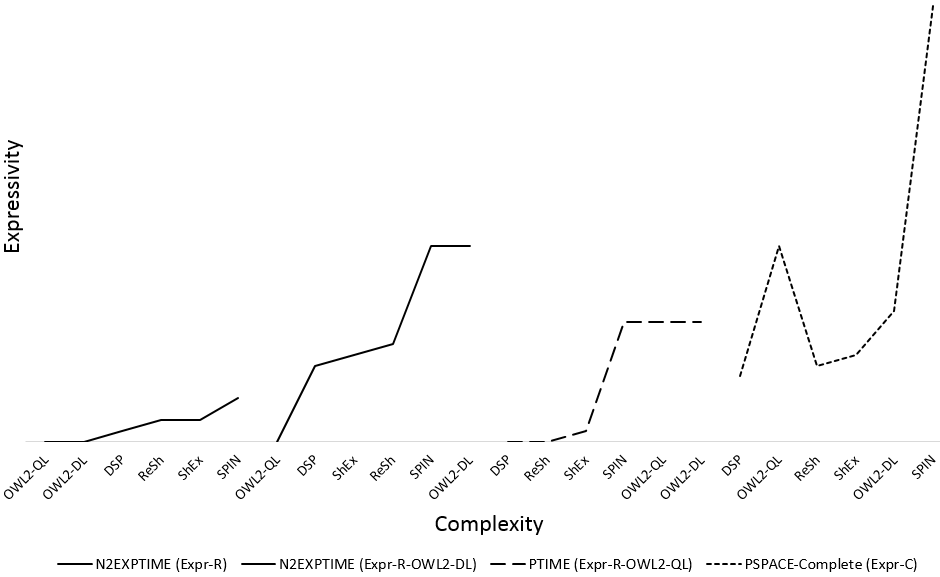
\includegraphics[width=1.00\textwidth]{expressivity-complexity-3.png}
	%\caption{Expressivity and Complexity}
	%\label{fig:expressivity-complexity}
%\end{figure}



%Expressivity and complexity classes can be combined in a diagram (see figure Figure~\ref{fig:expressivity-complexity}).

%\begin{figure}
	%\centering
		%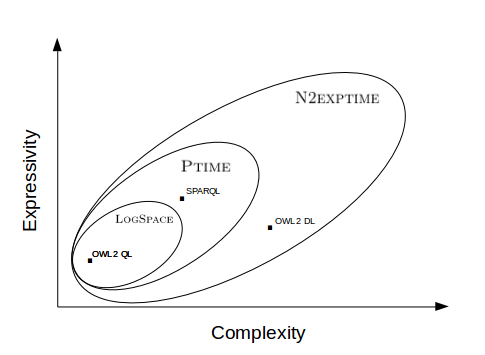
\includegraphics[width=0.95\textwidth]{complexiity_and_expressivity.png}
	%\caption{Complexity and Expressivity Classes}
	%\label{fig:expressivity-complexity}
%\end{figure}

%It depends on the individual use case, which constrains are needed to express and therefore which constraint language to choose.
%As a consequence, you may select a constraint language which is not the most expressive one within one specific expressivity class, 
%but may be better evaluated according to one or multiple user-friendliness classes.
%If, for instance, reasoning should not be performed and three particular constraints should be covered by the constraint language.
%Even if the absolute expressivity (\ms{Expr-C}) of SPIN is much higher than the one of ShEx (\ms{Expr-C}(ShEx) $\subset$ \ms{Expr-C}(SPIN)) 
%, the relative expressivity of this expressivity class could be the same for ShEx and SPIN - in case the three constraints are covered by both.
%\er{The expressivity here (in figure) is not constraint specific expressivity, it is more general. However, constraint specific expressivity must follow.}
%\tb{we need to create a new figure}
%Now, the user-friendliness classes comes into play:
%\begin{eqnarray*}
%\ms{UF-L}(SPIN) \subset \ms{UF-L}(ShEx), \ms{UF-I}(SPIN) \subset \ms{UF-I}(ShEx) \\
%\ms{UF-C}(SPIN) \subset \ms{UF-C}(ShEx), \ms{UF-L}(ShEx) \subset \ms{UF-L}(SPIN)
%\end{eqnarray*}
%Although, SPIN is more adopted than ShEx, ShEx is a high-level compared to a low-level language, ShEx is more intuitive and concise than SPIN.
%According to this evaluation, tools may recommend alternatives to the most expressive language SPIN.  

%\section{Implementation}
%\label{Implementation}
%
%SPARQL is generally seen as the method of choice to validate RDF data according to certain constraints, although it is not ideal for their formulation. 
%In contrast, OWL 2 DL constraints are comparatively easy to understand, but lack an implementation to validate RDF data. However, reasoning in OWL supports the identification of inconsistencies, which is also known as ontology debugging \cite{stuckenschmidt2008debugging}. Despite the fact that inconsistency detection especially in DL has already been studied extensively, it is not sufficient for constraint validation.
%Bosch and Eckert\cite{BoschEckert2014-2} use SPIN as basis to define a
%validation environment in which the validation of any constraint language\footnote{the only limitation is that constraint languages must be represented in RDF} can be implemented by representing them in SPARQL. 
%The validation implementation of constraint languages is fully declarative,
%consisting of a mapping from a constraint language to SPIN in form of SPARQL CONSTRUCT queries.
%SPIN represents both the SPIN mappings and the SPARQL queries in RDF. 
%Within the validation environment, we fully implemented the validation of all OWL 2 DL\footnote{and therefore all OWL 2 QL constructs} constructs. 
%The implementation can be tested at \url{http://purl.org/net/RDFval-demo} and
%the OWL 2 SPIN mapping is maintained at \url{https://github.com/boschthomas/OWL2-SPIN-Mapping}.
%
%The developed constraint language classification according to the three dimensions expressivity, complexity, and user-friendliness leads to many possible extensions of the RDF validator and similar validation systems.
%Users may choose if they wish to execute reasoning as a pre-validation step and which reasoning axioms they want to use to express their inference rules.
%They may also select which constraints they need for their use cases.
%
%As we defined an ordering of constraint languages for each expressivity class, we assigned reasoning axioms and constraints to complexity classes, we evaluated constraint languages regarding multiple user-friendliness criteria, the validator can provide a list of constraint languages for which the expressivity is enough to express the wished constraints and axioms.
%The validator can also recommend a constraint language of that list whose user-friendliness is evaluated to be the highest according to the user-friendliness criteria.
%As reasoning may cause high complexity, the validator may show which axioms from the user's selection cause the determined complexity class 
%and it may provide solutions how to get to the next lower complexity class.

\section{Related Work}
\label{sec:related-Work}

Tao \cite{tao2012integrity} suggested an \emph{OWL 2 DL} extension to support integrity constraints 
which enables thereby the use of \emph{OWL 2} as a constraint language for validation under the \emph{CWA} by conjunctive query answering. 
Tao also provides a solution to explain and to repair integrity constraint violations.
Siren and Tao \cite{SirinTao2009} proposed an alternative semantics for \emph{OWL 2} using the \emph{CWA} 
so that it could be used to validate integrity constraints.
They examined integrity constraint semantics proposed in the deductive databases literature and adopted them for \emph{OWL 2}
by reducing the validation of integrity constraints to \emph{SPARQL} query answering by means of reasoners.
Although, the alternative semantics for \emph{OWL 2} is implemented in the \emph{Stardog} database\footnote{\url{http://stardog.com/}}, it was never submitted to a standards organization such as the \emph{W3C}.

In \emph{DL}, reasoning tasks like query answering or detection of inconsistencies require the consideration of knowledge that is not only defined explicitly but also implicitly. To do so there are two different ways called forward- and backward-chaining. 
The first method implies a materialized knowledge base, where the original knowledge base is extended by all assertions that can be inferred. State-of-the-art \emph{DL} or \emph{OWL} reasoners following this approach are \emph{FaCT++} \cite{tsarkov2006fact++}, \emph{Pellet} \cite{sirin2007pellet},  \emph{RacerPro} \cite{haarslev2001racer}, or \emph{HermiT} \cite{horrocks2012hermit}. 

On the second approach, the original knowledge base is kept in its original state.
Before queries are evaluated against the knowledge base, the queries are rewritten such that the rewritings also consider the implicit knowledge in the result set. 
Approaches following this way are \emph{PerfectRef} given by Calvanese et al. \cite{Calvanese2007} or \emph{TreeWitness} proposed by Kontchakov et al. \cite{kontchakov2011combined}, which are both implemented in the --ontop-- framework\footnote{\url{http://ontop.inf.unibz.it}} for ontology-based data access. 
The first solution is applied on local knowledge bases whereas the second is more appropriate for federative environments like in \cite{nolle2014efficient,nolle2013elite}. 
%So, even if reasoning is performed by query rewriting in terms of backward-chaining and constraint validation queries are evaluated through such an engine, rewritings will only be generated if possible and will not affect constraint validation that are checked e.g. by pattern matching.


% additional papers
% -----

%Axel Polleres, Cristina Feier, and Andreas Harth. Rules with
%contextually scoped negation. In Proceedings of the 3rd European
%Semantic Web Conference (ESWC2006), volume 4011 of Lecture Notes in
%Computer Science (LNCS), pages 332-347, Budva, Montenegro, June 2006.
%Springer.
%
%And additionally:
%http://www2.informatik.uni-freiburg.de/~mschmidt/docs/sparql_constraints.pdf

\section{Conclusion and Future Work}

\begin{itemize}
	\item \textcolor{blue}{ToDo}
\end{itemize}

%In section \ref{the-role-of-reasoning-for-rdf-validation} we explained why reasoning is beneficial for validation and how reasoning interacts with validation.
%In section \ref{classification-rdf-constraints} we classified constraints according to CWA/UNA dependency, reasoning, and complexity.
%Constraint types can either be dependent on the CWA with UNA ($\mathcal{C}_{CWA}$), when it makes a difference if the CWA/UNA or the OWA/nUNA is assumed, or independent on the CWA with UNA ($\overline{\mathcal{C}_{CWA}}$).
%We distinguish two disjoint sets of constraint types $\mathcal{C}_{R}$ ({\em constraints with reasoning}) and $\overline{\mathcal{CT}_{R}}$ ({\em constraints without reasoning}).
%For each of them, we presented representative constraint types to investigate the effects of reasoning to the validation process.
Regarding the performance of constraints, we refer to worst case complexity.

%We divide $\mathcal{CT}_R$ into two not disjoint classes ($\mathcal{C}_R ^{\mathcal{QL}} \subseteq \mathcal{C}_R ^{\mathcal{DL}}$) for the validation by query answering with OWL 2 QL and OWL 2 DL reasoning respectively.
%It is well known that performing SPARQL queries is in \textsc{Pspace}-Complete \cite{Perez2009}, 
%which is assigned to $\overline{\mathcal{C}_R}$ (validation by query answering without reasoning).

%In section \ref{classification-constraint-languages} we classified constraint languages according to expressivity scores and classes. 
%An interesting result is that in terms of expressivity on constraint types, 
%all constraint languages can be fully covered by SPIN (except one constraint type which is partly implemented).
%All supported constraint types are already implemented by particular constraint languages (except for SPIN).

%Another important finding is that, none of other languages covers the other so far in terms of expressivity.

We use \emph{SPIN}, 
a \emph{SPARQL}-based way to formulate and check constraints, as basis to develop a
validation environment\footnote{Online demo available at \url{http://purl.org/net/rdfval-demo}, source code at: \url{https://github.com/boschthomas/rdf-validator}} to validate RDF data according to constraints expressed by arbitrary constraint languages\footnote{SPIN mappings available at: \url{https://github.com/boschthomas/rdf-validation/tree/master/SPIN}} \cite{BoschEckert2014-2}.

The \emph{RDF Validator} can directly be used to validate arbitrary RDF data for the three vocabularies. Additionally, own constraints on vocabularies can be defined using several constraint languages.

%Although accessible within our validation tool, we provide all implemented constraints\footnote{\url{https://github.com/boschthomas/rdf-validation/tree/master/constraints}} in form of SPARQL CONSTRUCT queries.
The \emph{SPIN} engine checks for each resource if it satisfies all constraints, which are associated with its assigned classes, and generates a result RDF graph containing information about all constraint violations.
There is one \emph{SPIN} construct template for each constraint type.
A \emph{SPIN} construct template contains a \emph{SPARQL CONSTRUCT} query which generates constraint violation triples indicating the subject and the properties causing constraint violations, and the reason why constraint violations have been raised.
A \emph{SPIN} construct template creates constraint violation triples if all triple patterns within the \emph{SPARQL WHERE clause} match.

We implemented the validation of all \emph{OWL 2 QL}, \emph{OWL 2 DL}, \emph{DSP} (and major \emph{ReSh} and \emph{ShEx}) constructs
within our \emph{SPIN} validation environment in form of \emph{SPARQL CONSTRUCT queries} (\url{http://purl.org/net/RDFval-demo}).
%\cite{BoschEckert2014-2}\footnote{SPIN mappings: \url{https://github.com/boschthomas/OWL2-SPIN-Mapping}, \url{https://github.com/dcmi/DSP-SPIN-Mapping}}.
For $\mathcal{R}$ constraint types (represented in \emph{OWL 2 DL}), you can choose if reasoning should be performed prior to validation.

As part of future work we will extend our validator to provide a list of constraint languages for which the expressivity is enough to express selected constraint types.
The validator may also recommend one of these constraint languages having the highest expressivity score and lowest complexity.
As reasoning may cause high complexity, the validator may show which constraint types from the user's selection cause the higher complexity class 
and it may provide solutions how to get to the next lower complexity class. In this regard, it would be charming to have an estimation on which group of constraint types would demand what class of complexity. However, this is not an easy question, since complexity results are language specific and operational semantics is involved as well. Therefore, it is hard to maintain a general complexity result for a constraint type independent of the language chosen. Yet, providing an estimation for particular cases can still be straightforward.

\textcolor{red}{reviews:}
\begin{itemize}
	\item \textcolor{red}{logical semantics vs. notation}
	
	\begin{itemize}
			\item 
\textcolor{red}{This paper makes a confusion between notations and logical semantics.
It is not clear whether they consider RDF as a notation or as a data model with a logical semantics.
This makes a lot of difference because several ontological statements can be expressed in RDF notation, even complex OWL inclusion statements. Their logical semantics cannot be ignored, even for the practioners.
When they write <author, rdfs:range, Person>, this means precisely that they do not have to add explicitly for every triple <uri\_j, author, uri\_k> as many triples <uri\_k, rdf:type, Person>.
This is the interest of RDF triplestores: to allow incomplete description of data, while allowing reasoning to complete it.
Section 2 makes complicate this basic property for which a sentence in the introduction would have been sufficient.
BTW, it is completely misleading to say in introduction  "Reasoning is a promising solution as a pre-validation step to overcome this shortcoming": reasoning must be part of RDF data management as soon as RDFS statements are declared (otherwise, why would they be declared ?).}
    \item \textcolor{blue}{answer from Erman and Thomas: We use RDF as data model (with intended semantics) when performing reasoning with RDFS/OWL 2 semantics (OWA/nUNA) as well as for RDF validation and not just as a notation. We suggest using RDFS/OWL 2 semantics (OWA, nUNA) when performing reasoning (the original intention of RDFS/OWL 2) and we propose to take multiple languages into account (i.a. OWL 2) with different semantics (CWA, UNA) for the purpose to validate RDF data. Reasoning should be an optional step prior to validation. When reasoning is not wished to be performed, however, then omitted class assignment triples, e.g., must cause constraint violations as they are not intended to be inferred.} 
		\item \textcolor{blue}{question for Erman: How and where to tackle this issue in our paper?}
\end{itemize}
%	\item While gross numbers give some insight, if the paper listed which
%problems can be solved by each constraint language, it might allow
%readers more insight. 
%  \item Is there a useful grouping of the kinds of
%restrictions that can be stated by each language?  
	\item \textcolor{red}{A reader might want to see some lessons or experiences that could be learned from such a comparative study.}
\end{itemize}

%\section{Christian's Feedback}
%
%everybody, in the following some comments related to the paper draft
%given to me by Erman. Feel free to include these comments. Further, I
%woul prefer to be removed from the authors list, because I do not have
%the time to work on the paper and I'm in the current status not so very
%happy with it. Anyhow, I think guys will be able to improve it. So here
%are now my comments.
%
%There are too many different issues that are not presented in a well
%structured way / partially overlapping In particular there are two main
%contributions for which it is hard to understand their interdependencies.
%
%a) the role of reasoning for constraint validation
%b) the classification of the 74 constraint pattern in relation to the 5
%constraint languages
%
%Honestly, i do not understand why there are certain paragraphs at
%certain places and how this all goes together. I discussed several
%details with erman and maybe he can put something into the paper.
%
%Anyhow, here are some suggestions that make the paper stronger. At the
%moment I have a feeling that there is only a low chance for acceptance,
%even though I see that lots of work is in this paper.
%
%1) I recommend to join section 1+2. In this new intro section I
%recommend to put an example for RDF validation, really oriented at a
%real scenario. For example, a library wants to publish some datasets as
%RDF by extracting them from different relational databases. In oder to
%achieve high data quality some constraints are defined first on a very
%generic level written down some natural language sentences.  Now it
%needs to be decided which formalism to use in order to formally express
%these constraints and to check their validity. Moreover, it needs to be
%clarified what role reasoning play in this verification and publication
%process. This will perfectly fit as motivation for the contribution of
%the paper and the example can be easily be used at other places of the
%paper.
%
%I would then always come back to the running example from the beginning
%and always use constraints that would fit to this scenario. I know you
%like this darth vader stuff, however, it is better to have some real
%usecase in mind otherwise people always think this is only relevant for
%such toy examples.
%
%2) I cannot see the difference between C_R and C_R' (i use ' instead of
%this complement line above). I think this not explained well and it
%would help a lot if there is one or better two examples from the 74
%constraint pattern for C_R and C_R'. However, there should also be a
%clear definition "C_R [are] constraints without reasoning" is not even a
%correct sentence, or differently speaking: The border of reasoning vs
%not reasoning is not well defined, there exists not such a border. I try
%to explain som of my problems.
%- The way I understand it, the distinction is based on whether a
%constraint is translatable to an OWL construct or not. The example with
%the Literal Pattern Matching seems to go in that direction.
%- If the criteria is whether or not its translateable to some formalims,
%then the table on bottom of page 8 makes no sense, especially the first
%column. This indicates whether a constraint belongs in one or the other
%class is independently of some chosen formalism
%- Is the Literal Pattern Matching an example for the C_R class? If yes
%its a very untypical one if you think of reasoning. Mayb it can be
%expressed with OWL, but is uses something very specific which looks very
%mud linke non reasoning.
%... after thinking a while I have a feeling that there is no real
%dictsinction between  C_R and C_R'.
%
%3) MAYBE: I recommend to remove the section on user friendliness. In a
%scientific paper this can only be answered by a field study or some
%questionaires or something like this.
%
%4) The UNA and CWA are important aspects, however, in Section 4 nd 5
%they are not used anymore. I would expect that a constraint type can be
%independent of the CWA or it can make a difference. For example:
%
%ex1: An address is a field that stores a string and its end is substring
%that refers to a number.
%ex2: If someone is a mother, she has at least one child.
%ex3: If someone is a women, it cannot be a man.
%
%ex1 has nothing to do with CWA or UNA, if you accept the CWA or its
%opposite, it doe not nmake a difference here.
%ex2 depends on CWA, in the CWA setting a mother without an explictly
%stated child violates the constraint. In OWA its different, the mother
%withour explicitly stated child is not a problem. You just have an axiom
%that allows you to entail that there is an (unknown) child.
%ex3 again independent of CWA.
%
%I was really wondering how many of the 74 patterns are independent and
%how many are dependent? Note that you can give a very clear definition
%what independent means. You can say, For a given constraint, if there
%exist not RDF dataset that would be inconsistent under CWA and
%consistent under OWA or vice versa, then the constraint is independent
%of the CWA.
%
%5) Make the tables floating such that the have figure caption andnnumber
%and refer to these numbers from the text
%
%6) You should discuss the argumenst in Section 7 in the light of the
%library example given in he intro. The argumentation in this section is
%somewhat strange because this seems to touch the question whether to
%materialize explict or to keep tjis implicit. It is also strange why
%eactly the spefic constructs listed in the subsctions have been picked.
%
%... the last pages of the paper I have not been reading in details and I
%will not find the time to do this.
%
%This might be worth reading, the hint was just given from Heiner:
%
%Axel Polleres, Cristina Feier, and Andreas Harth. Rules with
%contextually scoped negation. In Proceedings of the 3rd European
%Semantic Web Conference (ESWC2006), volume 4011 of Lecture Notes in
%Computer Science (LNCS), pages 332-347, Budva, Montenegro, June 2006.
%Springer.
%
%And additionally:
%http://www2.informatik.uni-freiburg.de/~mschmidt/docs/sparql_constraints.pdf
%
%Best regards, Christian.



%
% The following two commands are all you need in the
% initial runs of your .tex file to
% produce the bibliography for the citations in your paper.
\bibliographystyle{abbrv}
\bibliography{../../literature/literature}  % sigproc.bib is the name of the Bibliography in this case
% You must have a proper ".bib" file
%  and remember to run:
% latex bibtex latex latex
% to resolve all references
%
% ACM needs 'a single self-contained file'!
%
%APPENDICES are optional
%\balancecolumns
%\appendix
%Appendix A
%\section{Headings in Appendices}
%The rules about hierarchical headings discussed above for
%the body of the article are different in the appendices.
%In the \textbf{appendix} environment, the command
%\textbf{section} is used to
%indicate the start of each Appendix, with alphabetic order
%designation (i.e. the first is A, the second B, etc.) and
%a title (if you include one).  So, if you need
%hierarchical structure
%\textit{within} an Appendix, start with \textbf{subsection} as the
%highest level. Here is an outline of the body of this
%document in Appendix-appropriate form:
%\subsection{Introduction}
%\subsection{The Body of the Paper}
%\subsubsection{Type Changes and  Special Characters}
%\subsubsection{Math Equations}
%\paragraph{Inline (In-text) Equations}
%\paragraph{Display Equations}
%\subsubsection{Citations}
%\subsubsection{Tables}
%\subsubsection{Figures}
%\subsubsection{Theorem-like Constructs}
%\subsubsection*{A Caveat for the \TeX\ Expert}
%\subsection{Conclusions}
%\subsection{Acknowledgments}
%\subsection{Additional Authors}
%This section is inserted by \LaTeX; you do not insert it.
%You just add the names and information in the
%\texttt{{\char'134}additionalauthors} command at the start
%of the document.
%\subsection{References}
%Generated by bibtex from your ~.bib file.  Run latex,
%then bibtex, then latex twice (to resolve references)
%to create the ~.bbl file.  Insert that ~.bbl file into
%the .tex source file and comment out
%the command \texttt{{\char'134}thebibliography}.
%% This next section command marks the start of
%% Appendix B, and does not continue the present hierarchy
%\section{More Help for the Hardy}
%The acm\_proc\_article-sp document class file itself is chock-full of succinct
%and helpful comments.  If you consider yourself a moderately
%experienced to expert user of \LaTeX, you may find reading
%it useful but please remember not to change it.
\balancecolumns
% That's all folks!
\end{document}
